\chapter{Self-expressive Dictionary Learning for Dynamic 3D Reconstruction} \label{ch:video_l1}

\section{Introduction}

Thanks to the rapid development of mobile technology, it has become common that many people use their own mobile cameras to capture a common event of interest, such as a concert or a wedding. These real-life videos and photos usually have the dynamic objects as the main focus of the scene. With the bursting growth of such crowd sourced data, it is of interest to develop methods of dynamic object 3D reconstruction that enables understanding and visualization of the captured events.

In this work, we target the problem of dynamic 3D object reconstruction from these unsynchronized videos. 
More specifically, the method takes as input multiple video streams without inter-sequence temporal information. The video streams could potentially have different, irregular, and unknown frame rates (see Figure \ref{fig:overview}). 
As output, the method reconstructs the 3D positions of sparse feature points at each time instance (e.g., Figure \ref{fig:first_image}). 
Dynamic object reconstruction from unsynchronized videos is a challenging problem due to various factors, such as unknown temporal overlap among video streams, possible non-concurrent captures, and dynamic object motion. Any of these factors impedes the valid reconstruction from traditional 3D triangulation, which relies on the assumption of concurrent captures or a static scene.


\begin{figure*}
\centering
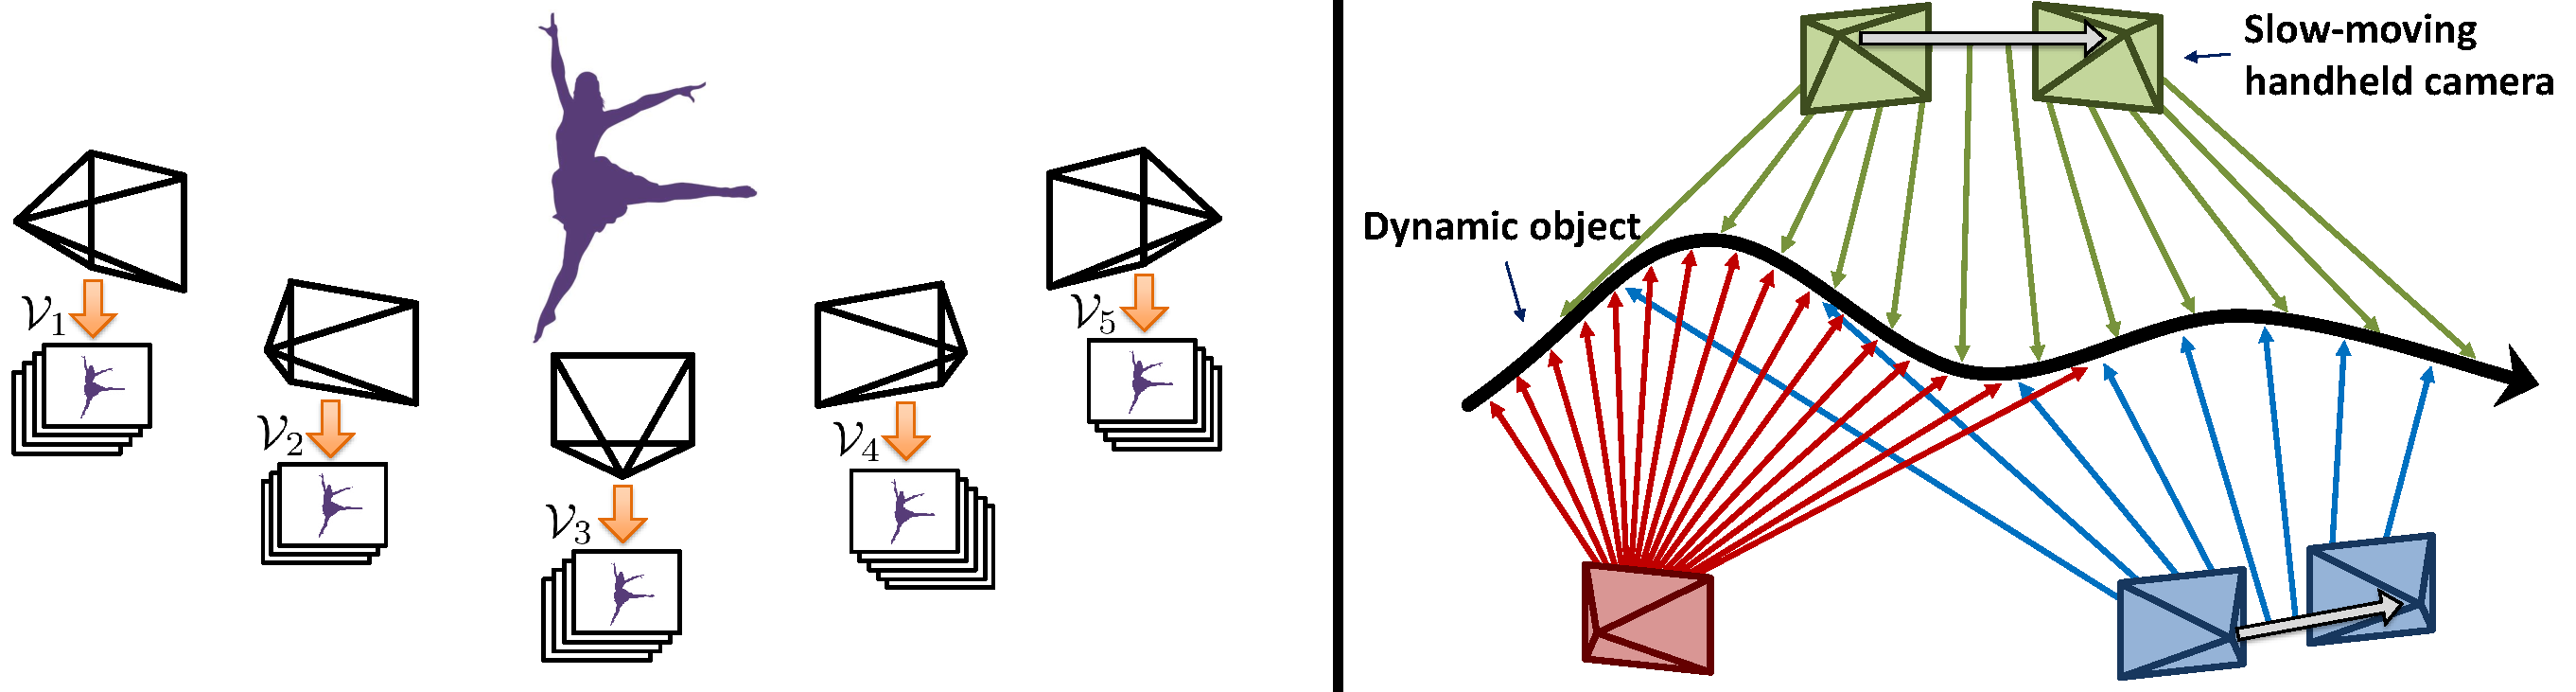
\includegraphics[width=1\textwidth]{chapter5/resource/overview_1_cropped.pdf}
\caption{\label{fig:overview} left: Multiple videos capture a performance.
The corresponding set of independent image streams  serves as input to our method.
Right: each input video has a different sampling of a 3D point's trajectory.}
\end{figure*}


Despite the ubiquity of uncontrolled video collections, there are currently no methods that can successfully address our problem.
Static scene reconstruction from photo collections has reached a high level of maturity~\cite{Snavely2,zheng2014patchmatch,Heinly} thanks to the development of structure from motion and depth estimation, but the reconstruction of dynamic objects using videos currently falls far behind the maturity of reconstruction of static scene elements. Existing methods of trajectory triangulation \cite{Park_ECCV2010, Valmadre_CVPR2012} from monocular image sequences inherently require temporal order information (sequencing information).
However, with independently captured videos, it is challenging to obtain this  information across videos. Zheng \etal~\cite{zheng2014joint} recently propose to jointly estimate the photo sequencing and 3D points by solving a generalized minimum spanning tree (GMST) problem. However, the NP-hard GMST problem itself limits the scalability of the approach. Also in this vein, the non-rigid structure from motion (NRSFM) problems have received extensive study over the two decades \cite{Tomasi_IJCV92,hartley2008perspective,dai2014simple}, but it is still under further exploration, especially if a perspective camera model is applied. 

To solve the problem, we observe that,
given the smooth motion of a dynamic object, any 3D shape at one time instance can be sparsely approximated by other shapes across time. 
Based on this self-expressive representation, our solution leverages the compressive sensing technique ($l_1$ norm), and tackles the problem in a dictionary learning framework \cite{aharon2006img,elad2006image}, where the dictionary is defined by the temporally varying 3D structure. Though the self-expression technique has been previously used in subspace clustering for motion segmentation \cite{elhamifar2009sparse}, and dictionary learning has been used in other applications such as image denoising \cite{elad2006image}, we are the first to explore learning a self-expressive dictionary for the problem of dynamic object reconstruction. 

\begin{figure}
\centering
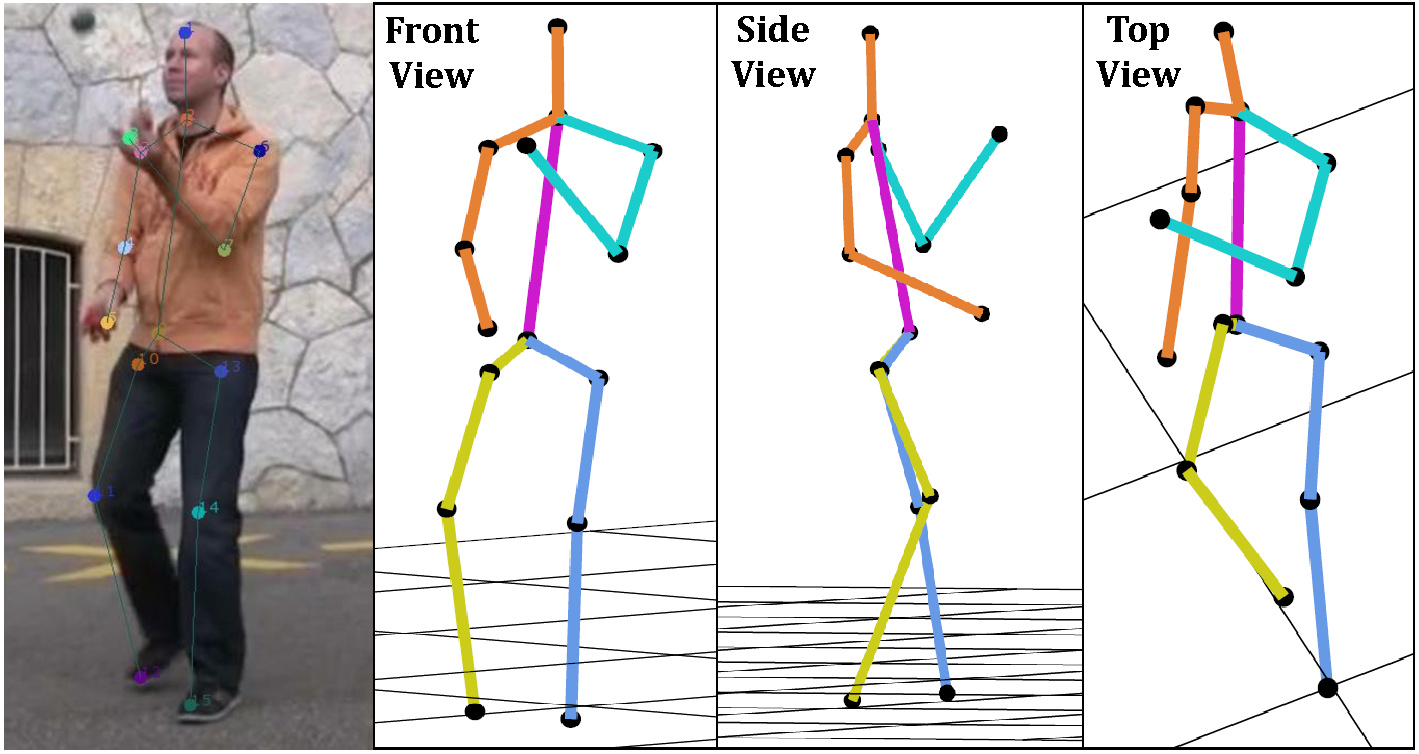
\includegraphics[width=0.75\textwidth]{chapter5/resource/first_image_cropped.pdf}
\caption{\label{fig:first_image}(left) Example frame from the multiple videos capturing a performance serving as input to our method, with overlaid structure (points), and (right three) different views of the reconstructed 3D points. Note our method only estimates the 3D points but no topology. The skeleton lines are plotted  for visualization purposes.}
\end{figure} 

The remainder of the work is organized as follows.
After introducing the notations in Section \ref{sec:problem_and_notations}, we begin describing foundations of our proposed approach in Section \ref{sec:principle}. Section \ref{sec:method} presents our model for dynamic object reconstruction without sequencing information, followed by the parameterization of the 3D structure given different kinds of 2D measures in Section \ref{sec:parameterization}.
Section \ref{sec:solver} describes our ADMM-based optimization solver to minimize the model. Then, Section \ref{sec:reconstructability} illustrates the reconstructablity of our algorithm. We provide experimental evaluations in Section \ref{sec:experiment}, and conclude the paper in Section \ref{sec:conclusion_l1}

%%%%%%%%%%%%%%%%%%%%%%%%%%%%%%%%%%%%%%%%%%%%%%%%%%%%%%%%%%%%%%%%%%%%%%%%%%%%%%%%%%%%%%%%%%%%%%%

%%%%%%%%%%%%%%%%%%%%%%%%%%%%%%%%%%%%%%%%%%%%%%%%%%%%%%%%%%%%%%%%%%%%%%%%%%%%%%%%%%%%%%%%%%%%%%%
\section{Problem and Notations} \label{sec:problem_and_notations}

We now describe the notations of our problem.
Let $\{\mathcal I\}$ denote an aggregated set of images attained from $N$ video sequences $\{\mathcal V_n \}$.
Assuming a total of $F$ available images, we can denote each individual image as $I_f \in \{\mathcal I\} $, where  $f=1,\dots,F$.
Alternatively, we can refer to  the $m$-th frame in the $n$-th video as $I_{(n,m)} \in\{\mathcal V_n \}$, where $n=1,\dots,N$ and $m=1,\dots, \left\vert{\{\mathcal V_n \}}\right\vert$.

We assume an {\em a priori} camera registration  through structure-from-motion analysis of  static background structures within the environment~\cite{WuVSFM}.
Accordingly, for each available image  $I_f$ we know the capturing camera's pose matrix
$\mathbf M_f=\left[  \mathbf{R}_f  \; |-\mathbf{R}_f \mathbf{C}_f\right]$,
along with its intrinsic camera matrix $\mathbf K_f$.

Without loss of generality, we first assume each image $I_f$ captures a common set of $P$ 3D points $\{\oneX_{(p,f)}~|~p=1,\dots,P\}$, and the 2D measure of each point is denoted as $\mathbf{x}_{(p,f)}$.
We also assume the correspondences of image measures $\mathbf{x}_{(p,f)}$ across images are available. 
Then for each measure $\mathbf x_{(p,f)}$, % with $p \in \{1, \dots, P \}$, 
we can compute a viewing ray with direction by 
\begin{equation}
\mathbf{r}_{(p,f)}=\mathbf{R}_f^{\text{T}} \mathbf{K}^{-1}_f 
\left[ 
\begin{matrix}   \mathbf{x}_{(p,f)} \\ 1  \end{matrix} 
\right],
\end{equation}
and followed by a normalization into a unit vector.

Hence, the position of the dynamic 3D point $\oneX_{(p,f)}$ corresponding to $\mathbf x_{(p,f)}$ can be described by the distance along the viewing ray $\mathbf{r}_{(p,f)}$ given by
\begin{equation}
\oneX_{(p,f)} = \mathbf{C}_f + d_{(p,f)} \mathbf{r}_{(p,f)},
\label{eq:X_representedBy_d}
\end{equation}
where % $\mathbf{C}_f$ is the camera center, $\mathbf{r}_{(f,p)}$ is the viewing directions, and
$d_{(p,f)}$
is the unknown distance of the 3D point from the camera center.

Given $F$ frames with each frame observing $P$ dynamic 3D points, we denote our aggregated observed 3D datum as
\begin{equation}
\label{eq:observationstructure}
\allX =
\begin{bmatrix}
\oneX_{(1,1)} & \cdots & \oneX_{(1,F)} \\
            \vdots  & \ddots & \vdots              \\
\oneX_{(P,1)} & \cdots & \oneX_{(P,F)} \\
\end{bmatrix} =
\left[
\shape_1\; \;  \cdots \; \;   \shape_F
\right]\;\;
\end{equation}
where the $f$-th column of the matrix $\allX$, denoted as $\shape_f$, is obtained by stacking all the $P$ 3D points observed in the $f$-th frame.

Then by defining $\allC$, $\allr$, and $\mathbbm{d}$ as follows,
\begin{equation}
\allC =
\begin{bmatrix}
\oneC_{1} & \cdots & \oneC_{F}
\end{bmatrix},
\end{equation}
\begin{equation}
\allr = 
\begin{bmatrix}
\oner_{(1,1)} & \cdots & \oner_{(1,F)} \\
            \vdots  & \ddots & \vdots              \\
\oner_{(P,1)} & \cdots & \oner_{(P,F)} \\
\end{bmatrix},
\end{equation}
\begin{equation}
%\mathbf{d} =
\mathbbm{d} =
\begin{bmatrix}
d_{(1,1)} & \cdots & d_{(1,F)} \\
            \vdots  & \ddots & \vdots              \\
d_{(P,1)} & \cdots & d_{(P,F)} \\
\end{bmatrix},
\end{equation}
Equation (\ref{eq:X_representedBy_d}) for all the points can be rewritten in matrix form as
\begin{equation}
\allX = \mathbf{1}_{P\text{x}1} \otimes \allC + 
(\mathbbm{d} \otimes \mathbf{1}_{3\text{x}1}) \odot \allr,
\label{eq:X_representedBy_d_all}
\end{equation}
where $\mathbf{1}_{P\text{x}1}$ is a $P$-by-$1$ matrix with values equal to 1, $\otimes$ is the Kronecker product, and $\odot$ is the component-wise matrix product. %(Hadamard product)

Our task is to recover  $\allX$ from the 2D measures without image sequencing information across the videos.

%%%%%%%%%%%%%%%%%%%%%%%%%%%%%%%%%%%%%%%%%%%%%%%%%%%%%%%%%%%%%%%%%%%%%%%%%%%%%%%%%%%%%%%%%%%%%%%%%%%%%%

%%%%%%%%%%%%%%%%%%%%%%%%%%%%%%%%%%%%%%%%%%%%%%%%%%%%%%%%%%%%%%%%%%%%%%%%%%%%%%%%%%%%%%%%%%%%%%%%%%%%%%

\section{Principle} \label{sec:principle}
The key observation driving our approach is that dynamic shape exhibits temporal coherence. In this section, we demonstrate how this principle can be leveraged to recover local temporal ordering with known shapes. Our proposed method will extend these ideas to situations with unknown structures.

For our method, we assume a smooth 3D motion under the sampling provided by the videos.
Hence, we can approximate the 3D structure  $\shape_f$ observed in image $f$ in terms of a linear combination of the structures corresponding to the set of immediately preceding ($\shape_{prev})$ and succeeding ($\shape_{next}$) frames in time.
That is, we have
\begin{equation}
\shape_f \approx w \cdot \shape_{prev} + (1-w) \cdot \shape_{next},
\label{eq:linear_comb_2}
\end{equation}
with $0 \leq w \leq 1$.
If our structure matrix $\allX$ from Equation (\ref{eq:observationstructure}) was temporally ordered, which it is not in general, the two neighboring frames would be $\shape_{f-1}$ and $\shape_{f+1}$.
Clearly, such perfect temporal order can be extracted from a single video sequence. However, the reconstructability constraints 
make single-camera structure estimation ill-posed (see Section \ref{sec:system_condition} for details). Hence, \textit{we rely on inter-sequence temporal ordering information to solve the dynamic structure estimation problem}. The absence of a global temporal ordering requires us to search for temporal adjacency relations across the different video streams having potentially different frame rates. 

In the most simple scenario, the pool of candidate neighboring frames is comprised by all other frames except $f$.
Writing the 3D points of the current frame $\shape_f$ as a linear combination of other frames, we have
\begin{equation}
\shape_f = \allX  \oneT_f,
\end{equation}
where $\oneT_f=\left(w_{(1,f)}, \dotsc, w_{(f-1,f)}, 0, w_{(f+1,f)}, \dotsc, w_{(F,f)}\right)^\text{T}$
is a vector of length $F$ representing the coefficients for the linear combination.
Note that the $f$-th element in $\oneT_f$ equals 0, since the $f$-th column of $\allX$ (corresponding to $\shape_f$) is not used as an element of the linear combination. 

Moreover,
since only a few shapes in the close temporal neighborhood of $\shape_f$ are likely to provide a good approximation, we expect the vector $\oneT_f$ to be sparse.
%Accordingly, we propose to find the most related 3D points through compressive sensing by introducing the $l_1$ norm as follows,
Accordingly, we propose to find the local temporal neighborhood of a shape $\shape_f$ through a compressive sensing formulation leveraging the $l_1$ norm:
\begin{equation}
\underset{\oneT_f}{\text{minimize}} ~ ||\shape_f - \allX \oneT_f||_2^2 + \lambda||\oneT_f||_1,
\label{eq:l1_orig}
\end{equation}
where $\lambda$ is a positive weight. Here, the $l_1$ norm serves as an approximation of the $l_0$ norm and favors the attainment of sparse coefficient vectors $\oneT_f$ \cite{bach2012optimization}.
Moreover,  we incorporate the desired properties of our linear combination framework (Equation (\ref{eq:linear_comb_2})) and reformulate Equation (\ref{eq:l1_orig}) as
\begin{equation}
\begin{aligned}
& \underset{\oneT_f}{\text{minimize}} && ||\shape_f - \allX\oneT_f||_2^2 \\
& \text{subject to} && \oneT_f \cdot \mathbf 1_{F\times 1}= 1 \\
&                   && \oneT_f \geq 0.
\end{aligned}
\label{eq:l1_new_equal}
\end{equation}
The affine constraints of Equation (\ref{eq:l1_new_equal}) constrain the variable $\oneT_f$ to reside in the simplex $\Delta_f$ defined as
\begin{equation}
\Delta_f \triangleq \{ \oneT_f \! \in \! \mathbb{R}^F \text{ s.t. } \oneT_f \! \geq \! 0, w_{(f,f)}=0 \text{ and } \sum_{j=1}^{F} w_{(j,f)} \! = \! 1 \}
\end{equation}

Despite the lack of an explicit $l_1$ norm regularization term in
Equation (\ref{eq:l1_new_equal}), as a variant of compressive sensing, it still keeps the sparsity-inducing effect \cite{bach2012optimization,chen:hal-00995911}. This is true for the present problem, since we know a shape can be well represented by temporally close shapes. A similar formulation has been used in modeling archetypal analysis for representation learning \cite{chen:hal-00995911}. There, the authors also provide a new efficient solver for this kind of problem.

Finally, we generalize our formulation from Equation (\ref{eq:l1_new_equal}) to include all available structure estimates $\shape_f$, with  $f=1,\dotsc,F$, into the following equation
\begin{equation}
\begin{aligned}
& \underset{\allT}{\text{minimize}}&& ~ || \allX - \allX \allT||_\text{F}^2\\
& \text{subject to} && \oneT_f \in \Delta_f, f=1,\cdots,F,
\end{aligned}
\label{eq:l1_given3D}
\end{equation}
where $||\cdot||_\text{F}$ denotes the Frobenius norm and $\allT=[\oneT_1 \dots \oneT_F]$ is an $F\times F$ matrix
with the $f$-th column equal to $\oneT_f$.
By construction, $\allT$ has all its diagonal elements equal to zero.

\begin{figure}
  \centering
  % Requires \usepackage{graphicx}
  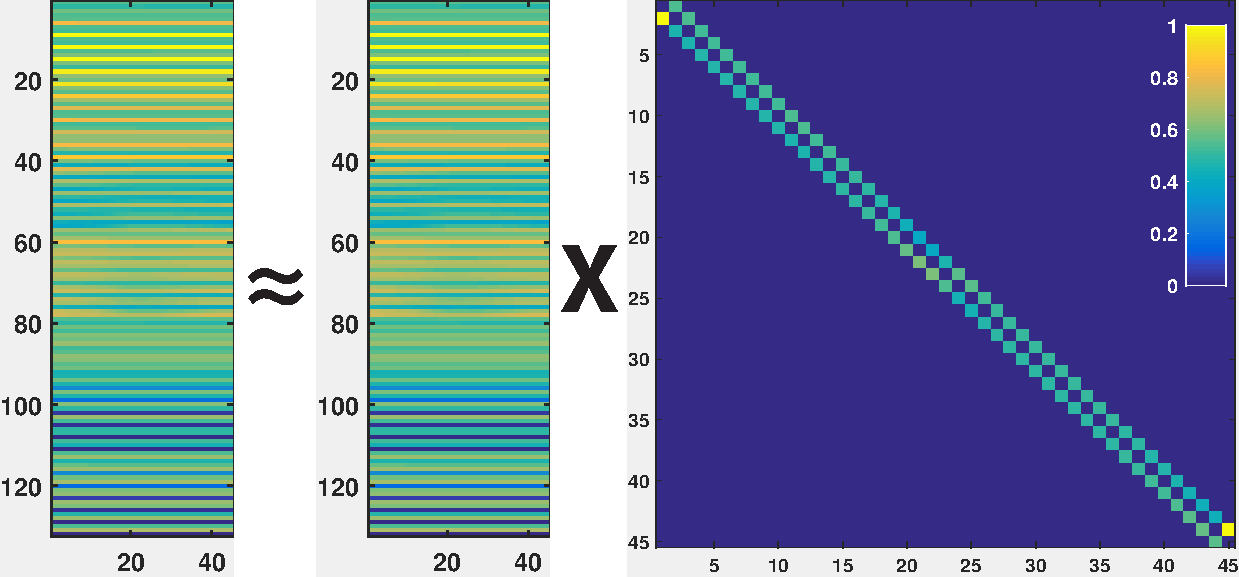
\includegraphics[width=0.95\textwidth]{chapter5/resource/l1.pdf}\\
  \caption{We illustrate the output of Equation (\ref{eq:l1_given3D}) on a real motion capture dataset ``Clap1Rep". 
For easy visualization, the shortest motion capture dataset (45 frames) presented in the work by \citet{cg-2007-2} is used. Each element/column in $\allX$  corresponds to  ground truth 3D structure. The estimation of $\allT$ through Equation (\ref{eq:l1_given3D}) approximates the correct ordering after enforcing all elements in the diagonal to be $0$.}
  \label{fig:principle}
\end{figure}

As an illustration of the validity of our compressed sensing formulation, Figure \ref{fig:principle} shows the output of Equation (\ref{eq:l1_given3D}) on a real motion capture dataset given known 3D points $\allX$. 
Although image sequencing is assumed unknown, we show results in temporal order for visualization purposes.
The coefficients in $\allT$ approximate a matrix having non-vanishing values only on the locations directly above and below the main diagonal.
This indicates that the 3D points $\shape_f$ are a linear combination of $\shape_{f-1}$ and $\shape_{f+1}$. 

Minimizing Equation (\ref{eq:l1_new_equal}) is equivalent to finding the most related shapes to linearly represent $\shape_f$. It is usually true that the temporally close shapes $\shape_{f-1}$ and $\shape_{f}$ are most related, and therefore local temporal information is recoverable from the non-vanishing values in $\allX$. However, if object motion is repetitive or if the object is static for a period of time, there is no guarantee that the most related shapes are the temporally closest ones. Even though this is true, the analysis in Section \ref{sec:shape_approximation} shows that this does not cause any problem for our method in regard to 3D reconstruction. 

To validate our prior of sparse representation for real motion, we quantitatively evaluate the estimated coefficients $\allT$ by minimizing Equation (\ref{eq:l1_given3D}) on all 130 real motion capture datasets presented in the work by \citet{cg-2007-2}. 
For a shape at a given time sample, we measure the sum of the two largest estimated coefficient values for this sample, and the frequency with which these top two coefficients correspond to the ground truth temporally neighboring shape samples. Given our prior, values of 1 for both measures are expected. The average values we obtain are 0.9972 and 0.9994, supporting the validity of our prior.


%%%%%%%%%%%%%%%%%%%%%%%%%%%%%%%%%%%%%%%%%%%%%%%%%%%%%%%%%%%%%%%%%%%%%%%%%%%%%%%%%%%%%%%%%%%%%%%%%%%%%%

%%%%%%%%%%%%%%%%%%%%%%%%%%%%%%%%%%%%%%%%%%%%%%%%%%%%%%%%%%%%%%%%%%%%%%%%%%%%%%%%%%%%%%%%%%%%%%%%%%%%%%
\section{Method}
\label{sec:method}

We address the problem of estimating sparse dynamic 3D structure from a set of spatially registered video sequences with unknown temporal overlap.
Section \ref{sec:principle} presented a compressive sensing formulation leveraging the self-expressiveness of all the shapes in the context of known 3D geometry.
However, our goal is to estimate the unknown structure without sequencing information.
To this end, we define our dictionary as the temporally varying 3D structure and propose a compressive sensing framework which poses the estimation of 3D structure as a dictionary learning problem.
We solve this problem in an iterative and alternating manner, where we optimize for 3D structure while fixing the sparse coefficients, and {\em vice versa}.
This is achieved through the optimization of a biconvex cost function that leverages the compressed sensing formulation described in Section \ref{sec:principle}  and, additionally, enforces both structural dependence coherence across video streams and motion smoothness among estimates from common video sources.

\subsection{Cost Function}
To achieve the stable estimation of both the structure $\allX$ and the sequencing information $\allT$, we extend our formulation from Equation (\ref{eq:l1_given3D}) to the following cost function:
\begin{equation}
\begin{aligned}
& \underset{\allX, \allT}{\text{minimize}}&& ~ \frac{1}{FP} || \allX - \allX\allT||_\text{F}^2
 + \lambda_1\Psi_1(\allT) + \lambda_2 \Psi_2(\allX) \\
& \text{subject to} && \oneT_f \in \Delta_f, f=1,\cdots,F;
\end{aligned}
\label{eq:ourproblem_final}
\end{equation}
where $\Psi_1(\allT)$ and  $\Psi_2(\allX)$ are two convex cost terms regulating the spatial relationships between 3D observations within and across video streams. We also add the normalization term $FP$ to cancel the influence of number of frames and number of points per shape. Next, we describe each of the cost terms in detail.

\subsection{Dictionary Space Reduction in Self-representation}
The first cost term in Equation (\ref{eq:ourproblem_final}) serves to find shapes in the dictionary to sparsely represent each shape. The search space can be reduced if some elements of $\allT$ are forced to be 0. As mentioned, the diagonal elements of $\allT$ are forced to be 0, since a shape is not used to represent itself. Moreover, it is possible that if {\em a priori} knowledge of rough temporal information across video steams is available, we can also leverage the knowledge to reduce the search space.

In our solution, we explicitly enforce that the shape observed by one video is not used to represent the shape observed in the same video, because 
the reconstructibility analysis in Section \ref{sec:system_condition} shows such estimation is ill-posed. In our implementation, enforcing this constraint is achieved by not defining the corresponding variables in $\allT$ during the optimization.

\subsection{Coefficient Relationships: $\Psi_1(\allT)$}
As described in Section \ref{sec:principle}, a given structure $\shape_f$ in frame $f$ can be obtained from the linear combination of the 3D shapes captured in other frames. The coefficients or weights of the linear combination are given by the elements of the matrix $\allT$. In particular, the element in the $j$-th row and $f$-th column  of $\allT$ is denoted as $w_{(j,f)}$, and it describes the relative contribution (weight) from $\shape_{j}$ in estimating $\shape_{f}$.
Similarly, $w_{(f,j)}$ represents the contribution of $\shape_{f}$ towards the 3D points in $\shape_{j}$.
Accordingly, a value of $w_{(f,j)}=0$ indicates the absence of any contribution from $\shape_{f}$ to $\shape_{j}$, which is desired for tempo-spatially non-proximal 3D shapes.

We note that, if $\shape_{f}$ contributes to $\shape_{j}$, it means the two sets of points are highly correlated, which
further implies that  $\shape_{j}$ should reciprocally contribute to estimating $\shape_{f}$.
We deem this reciprocal influence within our estimation process as {\em structural dependence coherence} and develop a cost term that
contributes toward enforcing this property within the estimation of $\allT$.
We encode this relationship into our cost function as an additional term of the form % $\Psi_1$ in Equation 
\begin{equation}
\Psi_1(\allT) = \frac{1}{F} ||\allT-\allT^\top||_\text{F}^2
\end{equation}

A strict interpretation of the above formulation aims to identify symmetric matrices.
In general, the reciprocal influence between $\shape_{f}$ and $\shape_{j}$ does not imply symmetric contribution,
as the values of $w_{(f,j)}$ and  $w_{(j,f)}$ depend on the actual 3D motion being observed.
\begin{figure}
  \centering
  % Requires \usepackage{graphicx}
  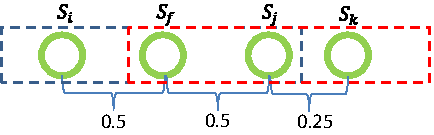
\includegraphics[width=0.75\columnwidth]{chapter5/resource/TripletFig.pdf}\\
  \caption{Illustration of the triplets influencing the weights for $\shape_f$ and $\shape_j$ leading to an asymmetric $\allT$. The values in the figure represent the distance between adjacent points.}
  \label{fig:Triplet}
\end{figure}
More specifically, these values describe the linear structural  dependencies between two different, but overlapping, 3-tuples of 3D points, e.g. ($\shape_{i}$,$\shape_{f}$,$\shape_{j}$) and ($\shape_{f}$,$\shape_{j}$,$\shape_{k}$) as illustrated in Figure \ref{fig:Triplet}. In the toy example of Figure \ref{fig:Triplet}, it can be seen that $\shape_{i}$ and $\shape_{j}$ are at equal distance to $\shape_{f}$ and hence equally contribute to it, i.e. $w_{(i,f)} = w_{(j,f)}=\frac{1}{2}$. However, in order to determine the linear combination weights for specifying $\shape_j$, we need to consider $\shape_f$ and $\shape_k$. Here, $\shape_f$ is twice as far from $\shape_j$ as $\shape_k$, and thus $w_{(f,j)}=\frac{1}{3}$, which is lower than $w_{(j,f)}$.
Accordingly, we do not expect a fully symmetric weight matrix   $\allT$. However,  given our expectation of a sparse coefficient matrix $\allT$, we can focus on finding congruence between the zero-value elements of the $\allT$ and $\allT^\top$, which $\Psi_1(\allT)$ effectively encodes.
Moreover, $\Psi_1(\allT)$  is convex, which enables its use within our biconvex optimization framework.
%But notice that  depending on the object motion, the amount of contributions can be different.

\subsection{Sequencing Information:$\Psi_2(\allX)$}

Under the assumption of sufficiently smooth 3D motion w.r.t.~the frame-rate of each video capture, we define a 3D spatial smoothness term that penalizes large displacements among successive frames from the same video.
Therefore, we define a pairwise term over the values of $\allX$
\begin{equation}
\Psi_2(\allX) = \frac{1}{M} \sum_{n=1}^{N}\sum_{m=1}^{\vert\mathcal V_n\vert-1}\left|\left|\oneX_{(n,m)} - \oneX_{(n,m+1)} \right| \right|_2^2
\end{equation}
where $n$ is the video index, $m$ is the image index within a video, $\vert \mathcal V_n\vert$ denotes the number of video frames within each sequence, and $M=\sum_{n=1}^{N}(\vert \mathcal V_n\vert - 1)$ is a normalization factor.
Note that $\Psi_2(\allX)$ does not explicitly enforce ordering information across video sequences, but instead fosters a compact 3D motion path within a sequence.
Moreover,  $\Psi_2(\allX)$ is a convex term.

However, this regularization term $\Psi_2(\allX)$ is a double-edged sword.
Since this term minimizes the sum-of-squared distances, if a video camera is static or has small motion, the estimated 3D points are likely to be pulled towards the camera center. 
This typically biases the estimated 3D points slightly away from their real positions. 
Therefore, we propose to first minimize Equation (\ref{eq:ourproblem_final}) until convergence to obtain values for $\allX$ and $\allT$, and then taking those values as initialization, we further optimize the problem with weight of $\Psi_2(\allX)$ (\ie $\lambda_2$) set to $0$.


%%%%%%%%%%%%%%%%%%%%%%%%%%%%%%%%%%%%%%%%%%%%%%%%%%%%%%%%%%%%%%%%%%%%%%%%%%%%%%%%%%%%%%%%%%%%%%%%%%%%%%

%%%%%%%%%%%%%%%%%%%%%%%%%%%%%%%%%%%%%%%%%%%%%%%%%%%%%%%%%%%%%%%%%%%%%%%%%%%%%%%%%%%%%%%%%%%%%%%%%%%%%%
\section{Parameterization of $\allX$} \label{sec:parameterization}

Given accurate 2D measurements, 
the 3D structures $\allX$ are constrained to lie on the viewing rays defined by the 2D measures and camera poses. Therefore, we can use Equation (\ref{eq:X_representedBy_d_all}) to represent $\allX$. This is deemed as a hard constraint, as the points have to lie on the viewing ray. However, in practice, the measures are typically noisy or unavailable due to, for example, inaccurate feature detection or motion blur. 
Next, we discuss the parameterization of $\allX$ given noisy and missing 2D observations.

\subsection{Noisy Observations} \label{sec:noisy_measure}
The parameterization using Equation (\ref{eq:X_representedBy_d}) enforces the hard constraint that 3D points lie on the viewing rays.%, but with noisy measures the viewing ray directions are inaccurate. 
Given that this may not be appropriate under the circumstance of noisy measurements, we can change this hard constraint to a soft constraint by adding a regularization term into the original Equation (\ref{eq:ourproblem_final}). Defining the objective function in Equation (\ref{eq:ourproblem_final}) as $\Phi(\allX,\allT)$, we propose a revised version as
\begin{equation}
\begin{aligned}
& \underset{\allX, \allT, \alld}{\text{minimize}} &&\Phi(\allX,\allT) + 
%\lambda_3 ||\mathbf{C} + \mathbf{r} \odot \mathbf{d} - \allX ||_F^2 \\
\lambda_3 ||\mathbf{1}_{P\text{x}1} \otimes \allC + (\mathbbm{d} \otimes \mathbf{1}_{3\text{x}1}) \odot \allr - \allX||_{\text{F}}^2 \\
 & \text{subject to} && \oneT_f \in \Delta_f, f=1,\cdots,F.
\end{aligned}
\label{eq:soft_constraint}
\end{equation}
The formulation converts the hard constraint of Equation (\ref{eq:X_representedBy_d_all}) as a soft constraint by adding a penalization if the 3D points deviate away from the viewing ray. The value of $\lambda_3$ controls how much a point can deviate away from the viewing ray, and it depends on the noise level of the 2D observations. A larger value should be used when the level of noise is lower. Note the new formulation is the same to the hard constraint if the weight $\lambda_3$ is set to $\infty$. Moreover, in Equation (\ref{eq:soft_constraint}), $\alld$ is an auxiliary variable solely depending on $\allX$. More details about the optimization of Equation (\ref{eq:soft_constraint}) are presented in Section \ref{sec:optimize_over_x}.
%The main drawback of this formulation is that it adds one more parameter $\lambda_3$.

\subsection{Missing Data} 
Each 3D point, given its accurate 2D measurement, lies on the viewing ray. Hence, the 3D point has one degree of freedom. However, in the absence of 2D observations, which can happen in the case of occlusion, the 3D points are no longer constrained by the viewing ray and thus have three degrees of freedom. 

In our method, the 3D points with missing 2D observations are interpolated by the estimated linear coefficients $\allT$. Therefore, this scheme is likely to produce larger errors if a dynamic 3D point is not observed by multiple consecutive frames across time. In our experiments, we test the accuracy of our algorithm under different missing-data rates.



%%%%%%%%%%%%%%%%%%%%%%%%%%%%%%%%%%%%%%%%%%%%%%%%%%%%%%%%%%%%%%%%%%%%%%%%%%%%%%%%%%%%%%%%%%%%%%%%%%%%%%

%%%%%%%%%%%%%%%%%%%%%%%%%%%%%%%%%%%%%%%%%%%%%%%%%%%%%%%%%%%%%%%%%%%%%%%%%%%%%%%%%%%%%%%%%%%%%%%%%%%%%%
\section{Optimization}\label{sec:solver}

The biconvex function in Equation (\ref{eq:ourproblem_final}) is non-convex, but it is convex if one set of the variables $\allX$ or $\allT$ is fixed.
Though a  more complicated dictionary update scheme such as K-SVD \cite{aharon2006img} is possible,
in this paper we use the simplest optimization scheme for Equation (\ref{eq:ourproblem_final}) that alternates the optimizations over $\allX$ and $\allT$.
Since the alternating optimization steps need to be performed until convergence, each step must be reasonably fast.
Although optimizing over $\allX$ is easy, optimizing over $\allT$ is relatively more difficult due to the simplicial constraint.
We find that optimizing over $\allT$ with a general solver, such as CVX \cite{cvx}, is too slow even for a moderate number of frames $F$.
Moreover, during our iterative optimization, the output of the previous step can be fed into the current step for better initializaiton (hot start), but typical general solvers, such as those based on interior point algorithm, do not allow for a hot start.
To solve the problem with speed and scalability, we propose a new solver based on alternating direction method of multipliers (ADMM) \cite{boyd2011distributed}.

\subsection{Optimize Over $\allX$} \label{sec:optimize_over_x}
If $\allT$ in Equation (\ref{eq:ourproblem_final}) is fixed, the optimization over $\allX$ is straightforward, as the problem is quadratic programming without any constraint, regardless of the difficulties discussed in Section \ref{sec:parameterization}.
\begin{enumerate}%[topsep=-1ex,itemsep=-1ex,partopsep=1ex,parsep=1ex]
\item {If the data are noise-free,
we can substitute Equation (\ref{eq:X_representedBy_d_all}) into Equation (\ref{eq:ourproblem_final}),
and obtain a quadratic programming problem without any constraint on the unknown variable $\alld$. }
\item{
In the case of noisy measurements, $\alld$ are dependent on $\allX$. More specifically, $d_{(p,f)}$ is given by
\begin{equation}
d_{(p,f)}=(\oneX_{(p,f)}-\mathbf{C}_{f})^\text{T}\mathbf{r}_{(p,f)}, 
\end{equation}
\ie~the projection of $\oneX_{(p,f)}-\mathbf{C}_{f}$ onto the viewing ray. Then, after replacing $\alld$ with $\allX$, we obtain a quadratic programming problem over unknown $\allX$.
}
\item{ For the case of missing observations, the corresponding 3D points are unknown variables. Therefore, for a given miss rate, the problem is quadratic over some unknown variables both in $\alld$ and in $\allX$.
}
\end{enumerate}
For the quadratic programming without constraints, the solution can be found at the zero value of the derivative of the cost function over the unknown variables.

\subsection{Optimize Over $\allT$} \label{sec:initlization}
The optimization over $\allT$ is more complex mainly due to the simplex constraints.
By fixing the variable $\allX$ in Equation (\ref{eq:ourproblem_final}), the cost function becomes,
\begin{equation}
\begin{aligned}
& \underset{ \allT }{\text{minimize}}&& ~ \frac{1}{FP} || \allX - \allX \allT||_\text{F}^2
 + \frac{\lambda_1}{F} ||\allT - \allT^\top||_2^2 \\
& \text{subject to} && \oneT_f \in \Delta_f, f=1,\cdots,F
\end{aligned}
\label{eq:ourproblem_TT}
\end{equation}
Notice that if the term $||\allT - \allT^\top||_\text{F}^2$ vanishes, the cost function is the same to Equation (\ref{eq:l1_given3D}). Equation (\ref{eq:l1_given3D}) can be decomposed into Equation (\ref{eq:l1_new_equal}), and optimized over $\oneT_f$ for each $f=1,\dots,F$ independently.
Therefore the number of variables for each subproblem is much smaller compared to the total number of variables in $\allT$, and it can be parallelized on the level of subproblems.
Moreover, \citet{chen:hal-00995911} propose a fast solver to the optimization problem in Equation (\ref{eq:l1_new_equal}) based on an active-set algorithm that can benefit from the solution sparsity.
However, the cost term $||\allT - \allT^\top||_\text{F}^2$ prevents the decomposition.

In this paper, we propose an ADMM algorithm that enables the decomposition.
By introducing a new auxiliary variable $\mathbb{Z}$, Equation (\ref{eq:ourproblem_TT}) can be rewritten as
\begin{equation}
\begin{aligned}
& \underset{ \allT }{\text{minimize}}&& ~ \frac{1}{FP} || \allX - \allX \allT||_\text{F}^2
 + \frac{\lambda_1}{F} ||\mathbb{Z} - \mathbb{Z}^\top||_\text{F}^2 \\
& \text{subject to} && \oneT_f \in \Delta_f, f=1,\cdots,F \\
&                   && \allT = \mathbb{Z}
\end{aligned}
\end{equation}
Though this change may seem trivial, the objective function is now separated in $\mathbb{W}$ and $\mathbb{Z}$. 
The ADMM technique allows this problem to be solved approximately by first solving for $\mathbb{W}$ with $\mathbb{Z}$ fixed, then solving for $\mathbb{Z}$ with $\mathbb{W}$ fixed, and next proceeding to update a dual variable $\mathbb{Y}$ (introduced below). This three-step process is repeated until convergence. Next, we describe each step of our ADMM-based algorithm. 

In step 1, $\mathbb{W}$ is updated by
\begin{equation}
\allT^{k+1}= \underset{\mathbf{T}_f \in{\Delta_f} \text{, for} 1\leq f\leq F}{\text{argmin}} \frac{1}{FP} ||\allX - \allX\allT||_\text{F}^2 + \text{vec}(\mathbb{Y}^k)^\top \text{vec} (\allT) + \frac{\rho}{2} ||\allT-\mathbb{Z}^k||_\text{F}^2,
\label{eq:step1}
\end{equation}
where the superscript $k$ is the iteration index. $\mathbb{Y}^k$ is the matrix of  dual variables and is initialized with 0. Note that the values of $\mathbb{Y}^{k}$ and $\mathbb{Z}^{k}$ are known during this step -- we only optimize over the variable $\allT$. The optimization can be decomposed into optimizing over $\oneT_f$ independently and in parallel, and we employ the fast solver proposed by \citet{chen:hal-00995911}. 

In step 2, we update the auxiliary variable $\mathbb{Z}$ according to
\begin{equation}
\mathbb{Z}^{k+1} = \underset{\mathbb{Z}}{\text{argmin }} \frac{\lambda_1}{F}||\mathbb{Z} - \mathbb{Z}^\top ||_\text{F}^2 - \text{vec}(\mathbb{Y}^k)^\top \text{vec}(\mathbb{Z}) + \frac{\rho}{2}||\allT^{k+1}-\mathbb{Z}||_\text{F}^2.
\label{eq:step2}
\end{equation}
This is a quadratic programming problem in the unknown variable $\mathbb{Z}$ without constraint and can be easily solved by setting the derivative of Equation (\ref{eq:step2}) with respect to $\mathbb{Z}$ equal to 0. 

In step 3, the dual variables $\mathbb{Y}$ are updated directly by
\begin{equation}
\mathbb{Y}^{k+1} = \mathbb{Y}^k + \rho(\allT^{k+1} - \mathbb{Z}^{k+1}).
\label{eq:step3}
\end{equation}
The three Equations (\ref{eq:step1}), (\ref{eq:step2}) and (\ref{eq:step3}) iterate until the stop criterion is met. We use the stop criterion described by \citet{boyd2011distributed}.

\subsection{Initialization of the Optimization}

Given the non-convexity of our original cost function (Equation (\ref{eq:ourproblem_final})), the accuracy of our estimates is  sensitive to the initialization values used by our iterative optimization. 
Hence, we design a 3D structure (i.e.~$\allX$) initialization mechanism aimed at
enhancing the robustness and accelerating the convergence of our biconvex framework.
While our approach explicitly encodes the absence of concurrent 2D observations, we aim to leverage the existence of nearly-incident corresponding viewing rays as a cue for the depth initialization of a given 3D point $\oneX_{(p,f)}$.
To this end, we identify for each bundle of viewing rays captured in $I_f$ (i.e. associated with a given shape structure $\shape_f$) an alternative structure instance captured at $I_j$ that minimizes the Euclidean 3D triangulation error across all corresponding viewing rays. In order to avoid a trivial solution arising from the small-baseline typically associated with consecutive frames of a single video, we restrict our search to ray bundles captured from distinct video sequences.

The position of each point $\oneX_{(p,f)}$ in $\shape_f$ is determined by $d_{(p,f)}$ as in Equation (\ref{eq:X_representedBy_d}).
Denoting $\mathbf{d}_f = [d_{(1,f)}, \dots, d_{(P,f)} ]$, we can find the  distance between
shapes of $\shape_f$ and $\shape_j$ by minimizing the following cost function over the unknown variables $\mathbf{d}_f$ and $\mathbf{d}_j$
\begin{equation}
\{\mathbf{d}_f^*,\mathbf{d}_j^*\} =  \underset{\mathbf{d}_f,\mathbf{d}_j } {\text{argmin}} ||\shape_f - \shape_j ||_2^2.
\label{eq:init}
\end{equation}
This is a quadratic cost function with a closed-form solution. % corresponding to the intersection points of each corresponding pair of viewing rays and their common normal.

We then build a symmetric distance matrix $\mathbf{D}$ with element $D_{(f,j)}$ equal to the minimum cost of Equation (\ref{eq:init}).
If the frames $f$ and $j$ are from the same video, $D_{(f,j)}$ is set to infinity.
%Next, we enforce cheirality constraints on the depth values, as we find many pseudo-intersection points with negative ray depth for spatio-temporally distant pairs of viewing rays.
Next, we find many pseudo-intersection points with negative ray depth for spatio-temporally distant pairs of viewing rays, and the corresponding element in $\mathbf{D}$ is also set to infinity.
Finally, we determine the minimum element of each $f$-th row in our distance matrix $\mathbf{D}$ and assign the corresponding depth values $\mathbf d^*_f$ as our initialization for the definition of our 3D structure $\mathbf{S}_f$.

\begin{figure}[]
\centering
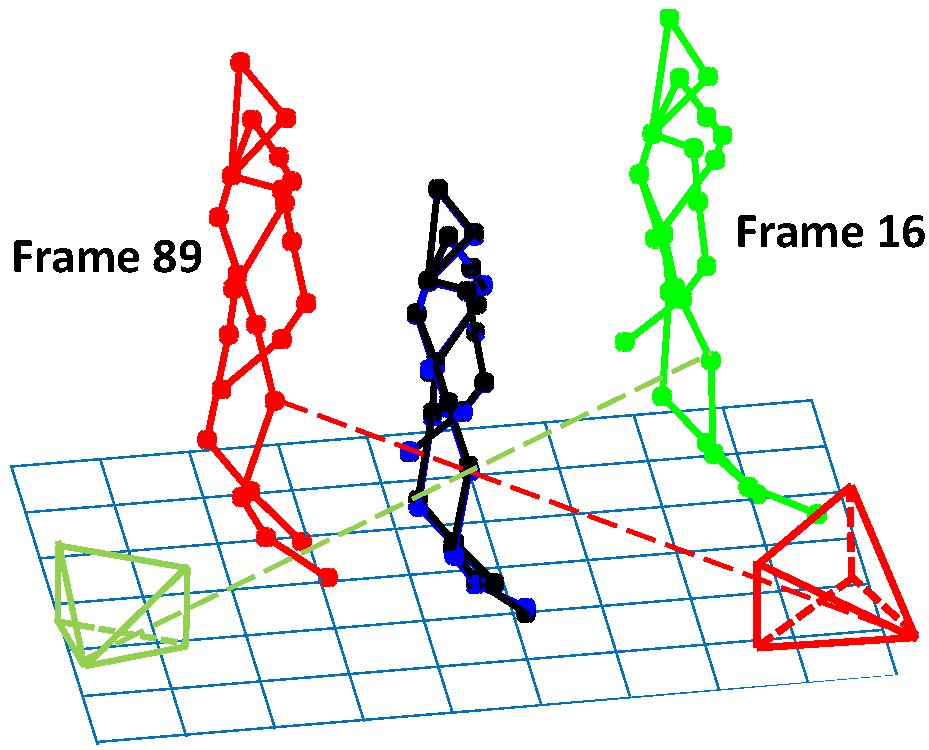
\includegraphics[width=0.70\textwidth]{chapter5/resource/wrong_init.pdf}
\caption{Example of incorrect initialization. The dataset `hopBothLegs3hops' \cite{cg-2007-2} has the motion of hopping forward three times. The black and blue shapes (almost overlapped) are the incorrect initialization of the real shapes (shown in green and red) of frames 16 and 89 due to the accidental ray intersections. This typically happens in the case of  periodic motion such as walking or jogging. In the figure, only one set of nearly intersecting rays is plotted.}
\label{fig:init}
\end{figure}

The above initialization is done regardless of available measurements, since we only look for an approximate initialization for the solver. In the case of missing data, the corresponding 3D points in the shape are simply ignored when minimizing Equation (\ref{eq:init}).

The output of the initialization is typically close to the ground truth, but may fail occasionally, as is shown in Figure \ref{fig:init}. This kind of wrong initialization may lead to wrong estimation of the two shapes if $\Phi_2(\allX)$ in Equation (\ref{eq:ourproblem_final}) is not present, because these two shapes can well represent each other. Our cost term $\Phi_2(\allX)$ helps to pull the occasional incorrect shapes out of local minima.


%%%%%%%%%%%%%%%%%%%%%%%%%%%%%%%%%%%%%%%%%%%%%%%%%%%%%%%%%%%%%%%%%%%%%%%%%%%%%%%%%%%%%%%%%%%%%%%%%%%%%%

%%%%%%%%%%%%%%%%%%%%%%%%%%%%%%%%%%%%%%%%%%%%%%%%%%%%%%%%%%%%%%%%%%%%%%%%%%%%%%%%%%%%%%%%%%%%%%%%%%%%%%
\section{Analysis and Discussion}	\label{sec:reconstructability}

%The reconstructability tells in which circumstances the algorithm \ref{eq:ourproblem_final} is able to recover the dynamic structure close to the ground truth. 
%From the analysis, it can be shown the importance of choosing neighboring shape associated with another video stream.
%The reconstructability of the algorithm describes the reconstruction accuracy under different capture scenario. 
%This sections starts from reconstructability analysis, 
%from where it is revealed why in our method the shape observed by one video is not used to represent the shape observed in the same video. 
%Moreover, we describes 
%Why sequencing information is not required in our method, while it is vital for all the other trajectory triangulation methods.
This section provides key insight to our algorithm for dynamic object reconstruction without sequencing. %The following important statements will be explained at length.
The following statements will be illustrated in detail.
\begin{enumerate}
\item To obtain good reconstructability, a shape observed by one video should not be used to represent the shape observed in the same video. 
\item To achieve accurate results, a 3D shape should be well approximated by other shapes.
\item While sequencing information is vital in other trajectory triangulation methods for structure estimation \cite{Park_ECCV2010,Valmadre_CVPR2012}, our method does not require it.
\end{enumerate} 
Next, we first describe the formulation of reconstruction errors by our method, based on which the above statements are illustrated at length in the subsequent three subsections.

\subsection{Representation of Reconstruction Errors}
Our solution computes 3D structure by minimizing the non-convex function Equation (\ref{eq:ourproblem_final}).
Since direct analysis of the non-convex function is difficult, we only analyze the problem with the assumption that the ground truth of $\allT$, which is defined as the output of Equation (\ref{eq:ourproblem_final}) given ground truth structure, is already known. 
%Our analysis reveals the effectiveness of our approach if a good $\allT$ is given. 
Without loss of generality, we also assume the 2D measures are noise-free.

Given that in our method $\lambda_2$ is set to 0 in the end, and $\allT$ is known and fixed, Equation (\ref{eq:ourproblem_final}) is equivalent to
\begin{equation}
\begin{aligned}
& \underset{\allX}{\text{minimize}}&& ~ || \allX - \allX\allT||_\text{F}^2 . 
\end{aligned}
\label{eq:recon_original}
\end{equation}
From Equation (\ref{eq:recon_original}), it can be seen when $\allT$ is fixed, all points in a shape are computed independently, and computing one 3D point per shape versus multiple points per shape basically follows the same routine. 
Therefore, for the sake of more concise presentation, the analysis in this section assumes only one point per shape, and the point index $p$ for the shape is omitted.

To analyze the reconstruction error, we assume that the ground truth of the 3D points is already known, and then analyze how much the computed structure deviates away from the ground truth, which is deemed as reconstruction error.
We denote the ground truth 3D point as
$\allX^*=[\oneX_1^*, \cdots, \oneX_f^*,  \cdots, \oneX_F^*]$. 
Then, any point $\oneX_f$ on the viewing ray that passes through $\oneX^*_f$ can be parameterized as 
\begin{equation}
\oneX_f = \oneX^*_f + l_f \mathbf{r}_f,
\label{eq:new_line_represent}
\end{equation}
where the unknown $l_f$ is the signed distance from the ground truth along the viewing ray. 

When minimizing Equation (\ref{eq:recon_original}), using either Equation (\ref{eq:new_line_represent}) or Equation (\ref{eq:X_representedBy_d}) to represent $\oneX_f$ actually 
generates the same 3D point, though the estimated values of $d_f$ and $l_f$ may not be the same. 
Therefore, $l_f$ represents the Euclidean error of our  method. 
%It means if $l_f$ equals 0, the dynamic 3D point is ideally reconstructed.

Equation (\ref{eq:recon_original}) is a quadratic objective function without any constraint and has a closed-form solution. We use Equation (\ref{eq:new_line_represent}) to represent the 3D point, and by setting the derivative of Eq.~(\ref{eq:recon_original}) over variables $\mathbf{l} = [l_1,\dots,l_f,\cdots,l_F ]$ to 0, we obtain a linear equation system denoted as
\begin{equation}
\mathbf{A}\mathbf{l} = \mathbf{b},	\label{eq:alb}
\end{equation}
where $\mathbf{A}$ is an $F \text{X} F$ matrix with the $f$-th row given by
\begin{equation}
\mathbf{A}_{:f} = (\mathbf{I}-\allT)_{:f}(\mathbf{I}-\allT)^\text{T} \text{diag}([\mathbf{r}^T_1 \mathbf{r}_f, \cdots, \mathbf{r}_F^T \mathbf{r}_f] ),
\label{eq:A}
\end{equation}
and $\mathbf{b}$ is an $F \text{X} 1$ vector with the $f$-th element given by
\begin{equation}
%\mathbf{b}_{f} = \mathbf{r}_f^T[X^*_1,\dots,X^*_F] (\mathbf{I}-\allT) (I-\allT)_{:f}.
\mathbf{b}_{f} = \mathbf{r}_f^T \allX^* (\mathbf{I}-\allT) (I-\allT)_{:f}^{\text{T}}.
\label{eq:b}
\end{equation}
In Equations (\ref{eq:A}) and (\ref{eq:b}), the subscript $_{:f}$ denotes the $f$-th row of a matrix, and $\mathbf{I}$ is an identity matrix. Then the solution for $\mathbf{l}$ is
\begin{equation}
\mathbf{l} = \mathbf{A}^{-1}\mathbf{b}. 
\label{eq:a_minus_1_b}
\end{equation}
As mentioned, $\mathbf{l}$ is the reconstruction error, 
which is bounded by 
\begin{equation}
||\mathbf{l}||_2= ||\mathbf{A}^{-1} \mathbf{b}||_2 \leq ||\mathbf{A}^{-1}||_2 ||\mathbf{b}||_2.
\end{equation}
In this paper, we use the term reconstructability (first defined in \cite{Park_ECCV2010}) as a criterion to characterize the reconstruction accuracy of our algorithm. 
In our case, in order to achieve high reconstructability, $||\mathbf{A}^{-1}||_2$ and $||\mathbf{b}||_2$ should be small. Next, we discuss $||\mathbf{A}^{-1}||_2$ and $||\mathbf{b}||_2$ in detail.


\subsection{System Condition} \label{sec:system_condition}
\begin{figure*}[]
\centering
\subfloat[]{
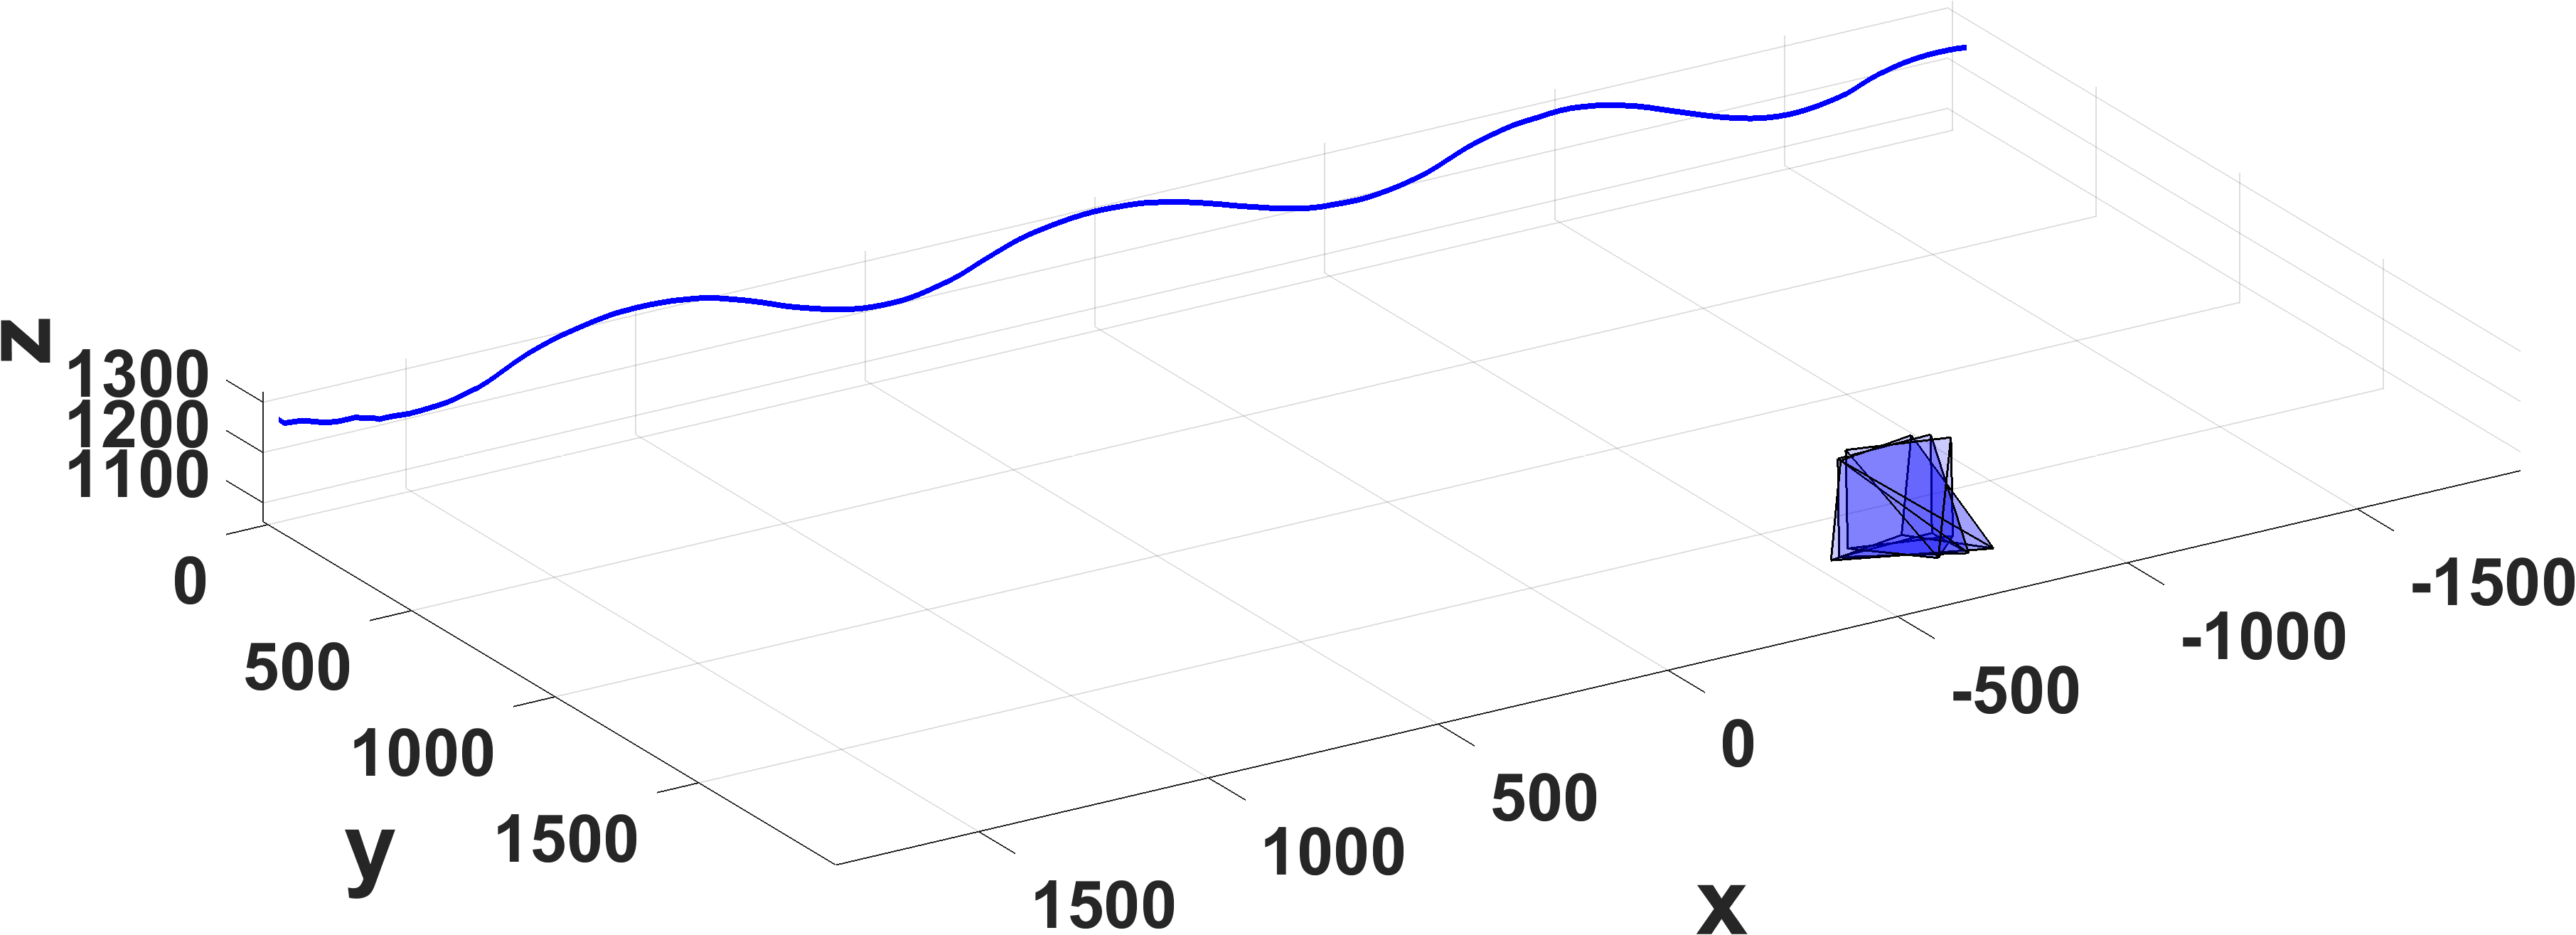
\includegraphics[width=0.86\textwidth]{chapter5/resource/one_cam.png}
\label{fig:oneCam}
}\\
\subfloat[]{
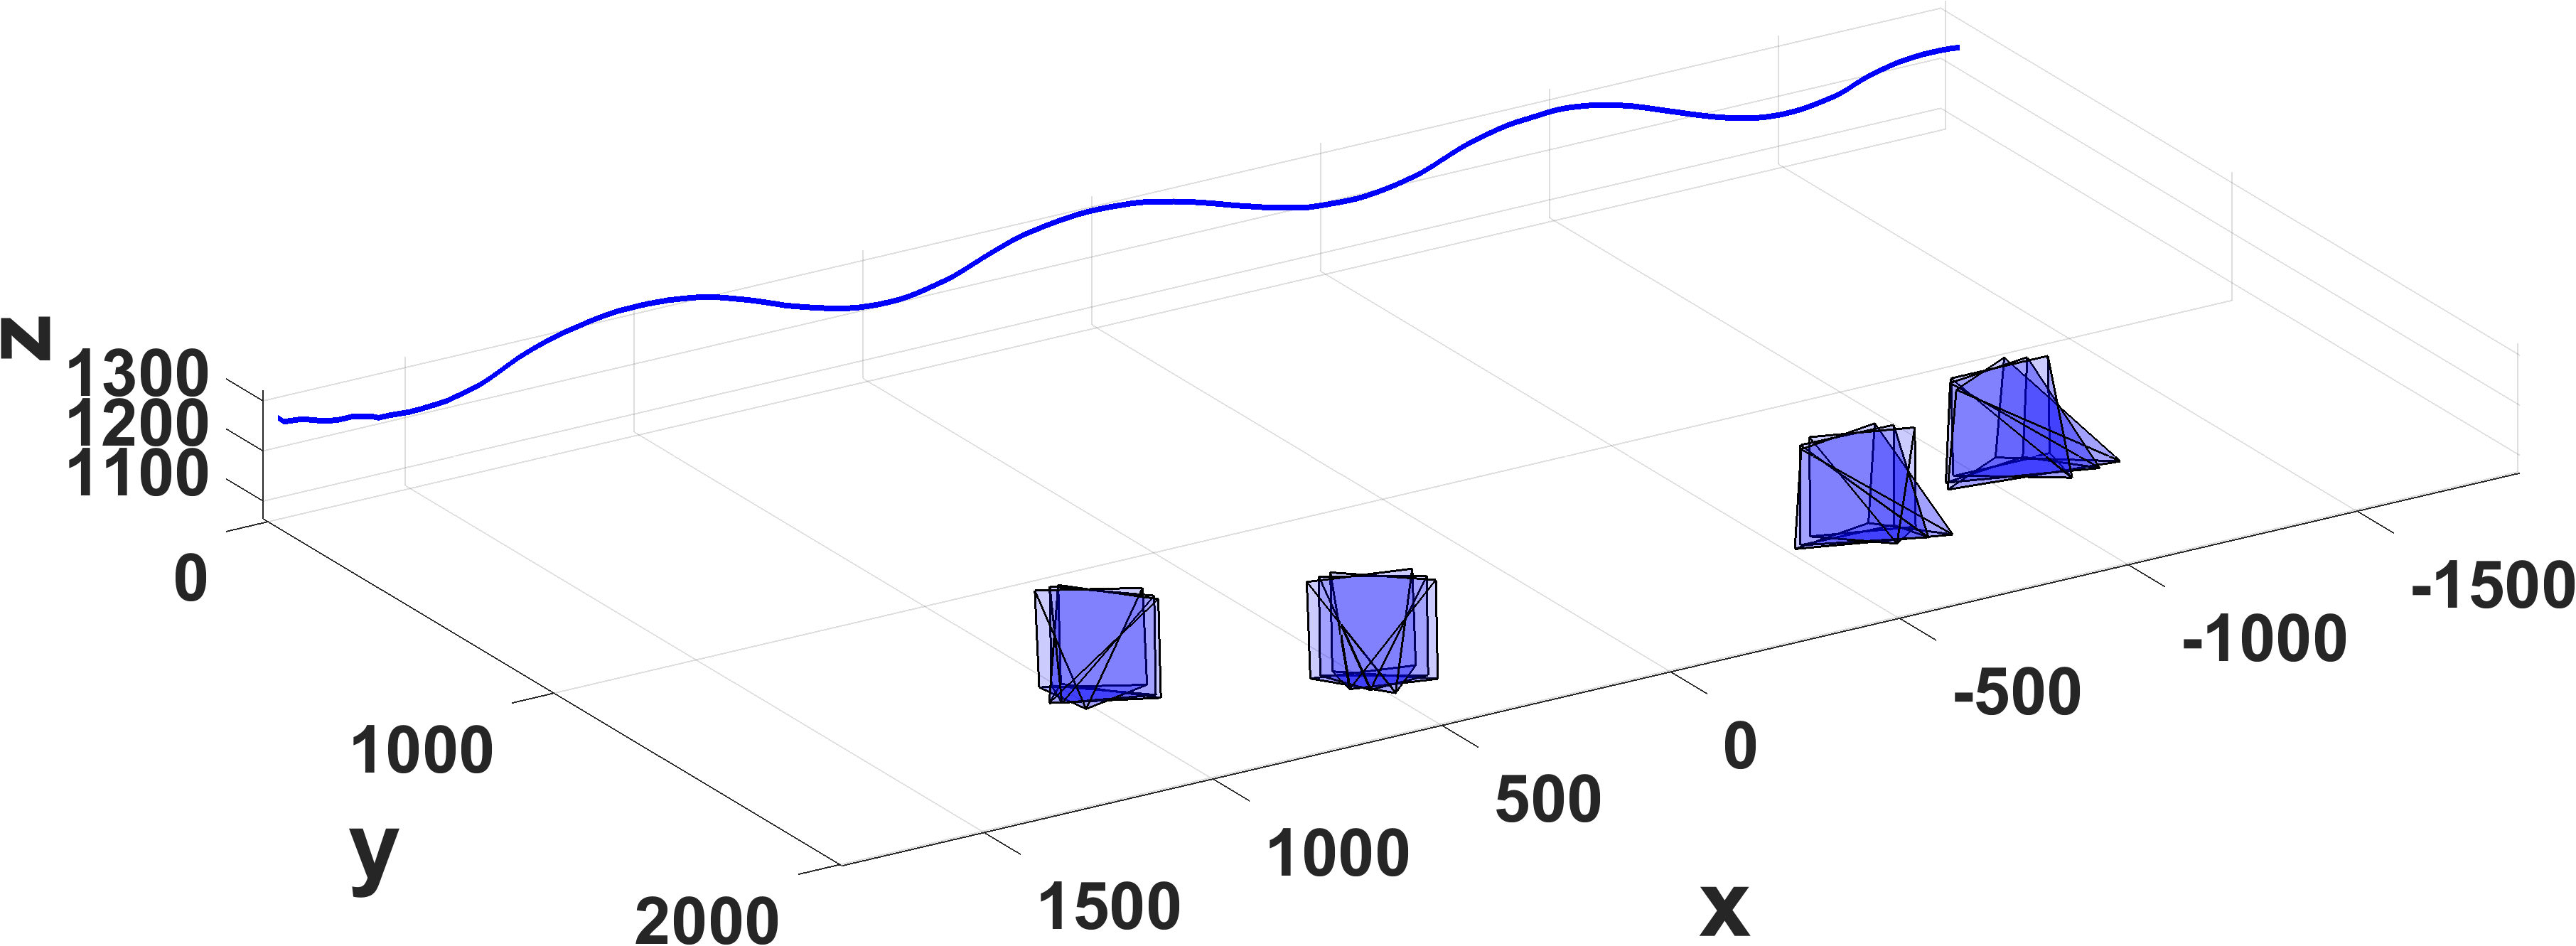
\includegraphics[width=0.86\textwidth]{chapter5/resource/multi_cam.png}
\label{fig:multiCam}
}\\
\subfloat[]{
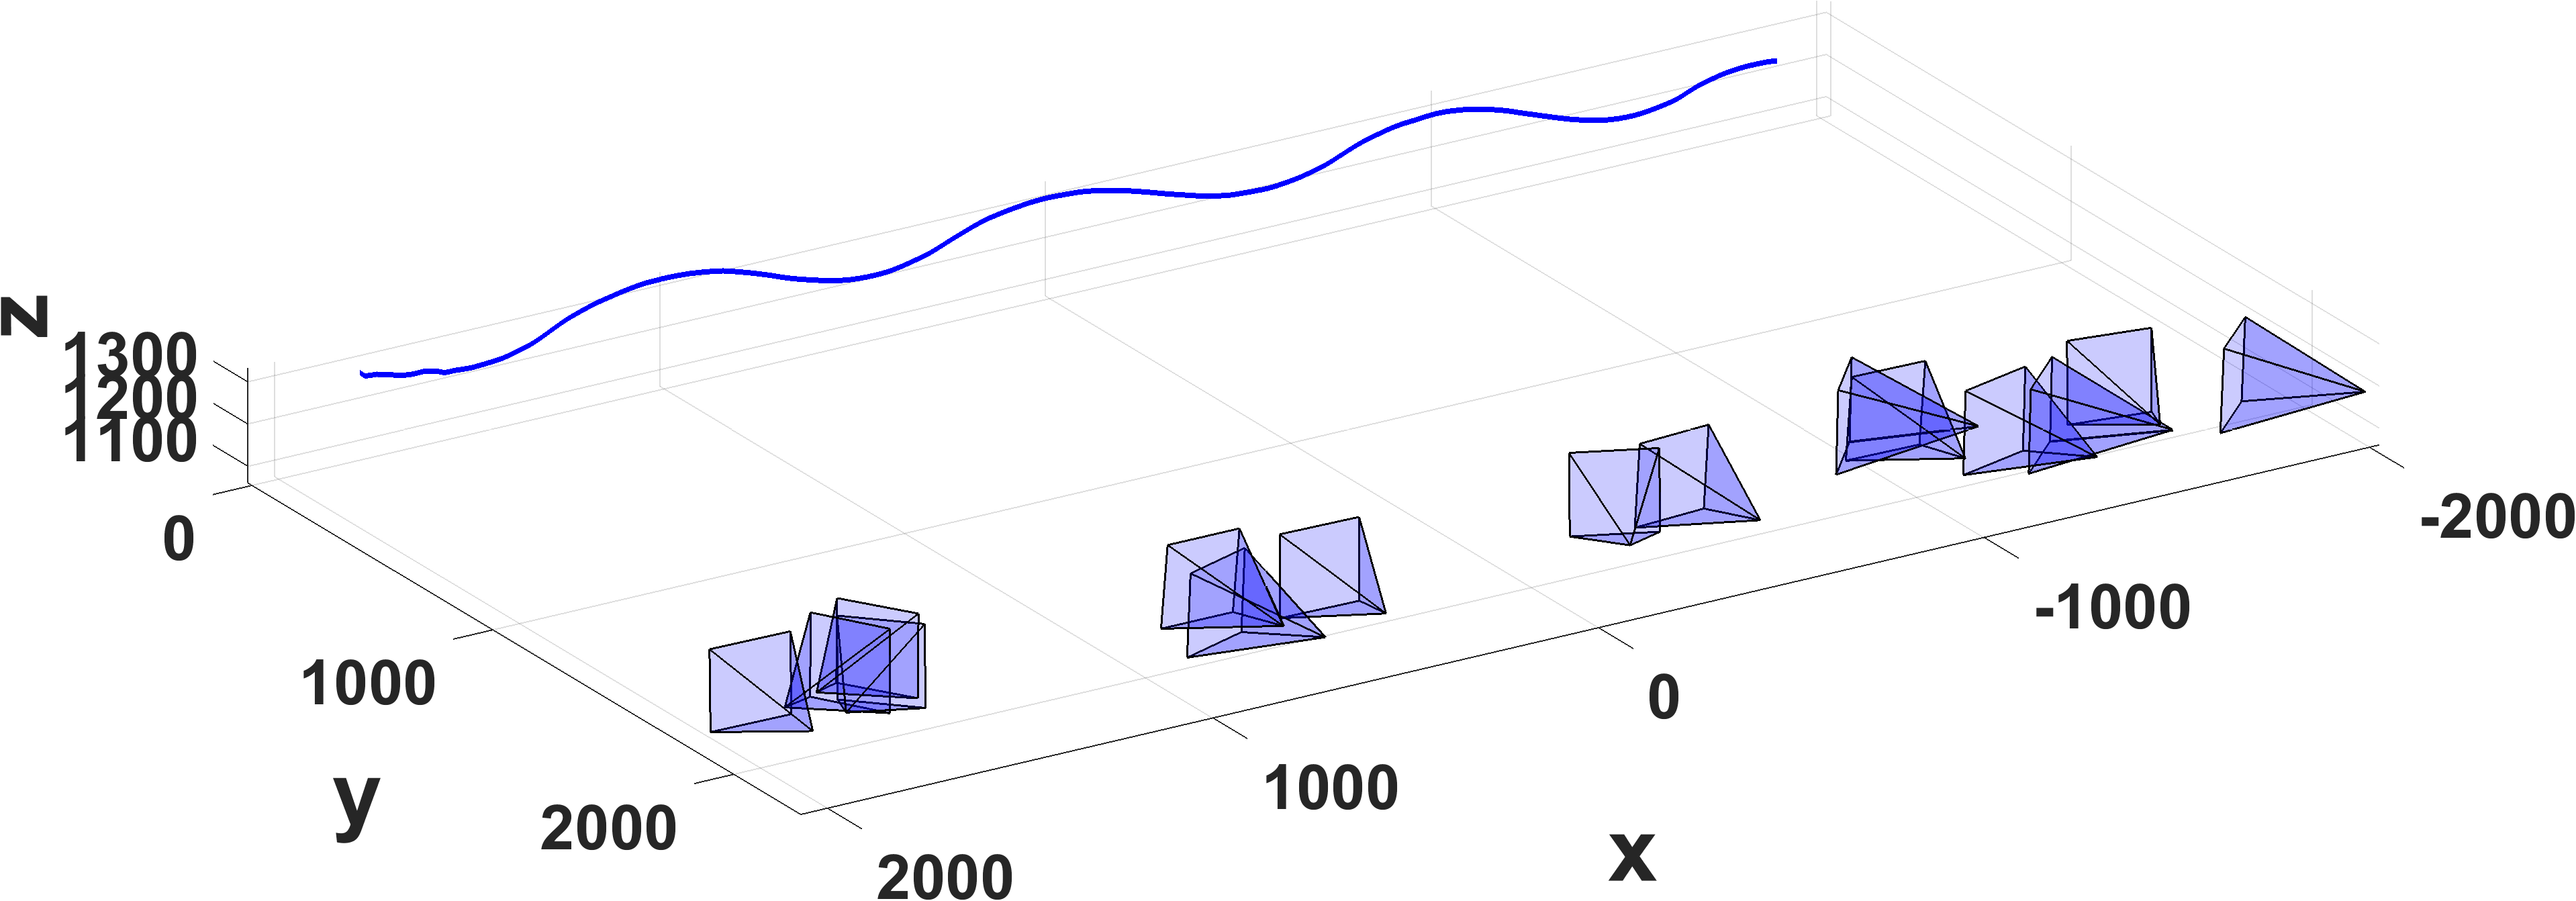
\includegraphics[width=0.86\textwidth]{chapter5/resource/random_cam.png}
\label{fig:randCam}
}\\
\caption{Simulated camera setups. The blue curve is a trajectory of a 3D point obtained from real motion capture data. Figures \ref{fig:oneCam} and \ref{fig:multiCam} show the slow-moving handheld cameras at three time instances. Figure \ref{fig:randCam} depicts a scenario where each camera only captures one image.
Figure \ref{fig:multiCam} and Figure \ref{fig:randCam} show the camera setups of our method and of the method by \citet{zheng2014joint}, respectively. Coordinates are in millimeters (mm).
}
\label{fig:condition}
\end{figure*}

Based on the definition of the matrix Euclidean norm, we have
\begin{equation}
||\mathbf{A}^{-1}||_2 = 1/\sigma_{\text{min}}, 
\label{eq:sysCondition}
\end{equation}
where $\sigma_{\text{min}}$ is the smallest singular value of matrix $\mathbf{A}$. 
With fixed $\allT$, we observe from Equation (\ref{eq:A}) that $\mathbf{A}$ solely relies on the viewing ray directions and does not depend on the exact positions of the 3D points $\allX^*$ along the viewing rays.
%Moreover, for a certain type of object motion, the viewing ray directions mainly depend on the camera setup. For instance, the dynamic scene captured by one handheld camera with small motion has very different $\sigma_{\text{min}}$ from that captured by multiple cameras with large baseline. 
Since $\sigma_{\text{min}}$ is closely related to reconstruction errors and is determined by the camera system setup, we call it system condition. 
Note the system condition introduced here is in essence very similar to the system condition number described in the works \cite{Valmadre_CVPR2012,zheng2014joint}.

Since direct analysis of the system condition given viewing ray directions $\{\mathbf{r}_1,\dots,\mathbf{r}_F\}$ based on Equation (\ref{eq:A}) is difficult, we next use empirical simulation to demonstrate the system condition under different camera setups. %as is shown in Figure \ref{fig:condition}. 

In the experiments, we simulate scene captures close to real life.
We use motion capture datasets that sample the 3D structure of real dynamic objects at 40 Hz. 
Figures \ref{fig:oneCam} and \ref{fig:multiCam} simulates setups of one handheld camera and multiple handheld cameras that record videos of a person walking. 
To mimic small random motion in each handheld camera, 
the camera centers at different time instances are Gaussian with standard deviation of 10 mm around a fixed center. 
We also test the case of completely random cameras (Figure \ref{fig:randCam}), with each taking one photo. %This camera setup is used in \cite{zheng2014joint}.  
The 3D structure at each time instance is projected to one of the virtual cameras to generate a set of 2D observations. For the scenario in Figure \ref{fig:multiCam}, we ensure no two shapes at consecutive time instances are projected into the same video stream.

We estimate the system condition using Equation (\ref{eq:sysCondition}) on 500 trials with random cameras. 
The average system conditions for the cases of Figures \ref{fig:oneCam}, \ref{fig:multiCam} and \ref{fig:randCam} are 1.48e+04, 22.3, and 29.0 respectively. It is evident the setup with one handheld camera has very low reconstructability.
Note that even though system conditions of camera setups in Figures \ref{fig:multiCam} and \ref{fig:randCam} are favorable, sequencing information for these two cases is not readily available.

To illustrate that the shape observed by one video should not be used to represent the shape observed in the same video (statement 1), we conduct an experiment to show the system condition if the observations from different video streams do not interleave. As shown in Figure \ref{fig:frameDist}, the dynamic object is observed by one camera for $N$ frames, and then observed by another camera for $N$ frames. We show empirically that as $N$ increases, the system condition increases monotonically, which indicates larger reconstruction error. If statement 1 is not met, it is likely the consecutive observations from the same video stream are used. This results in a large system condition and hence low reconstructability, even under the assumption that $\allT$ can be correctly estimated.

\begin{figure}[]
\centering
\subfloat[Observation without overlap]{
\centering
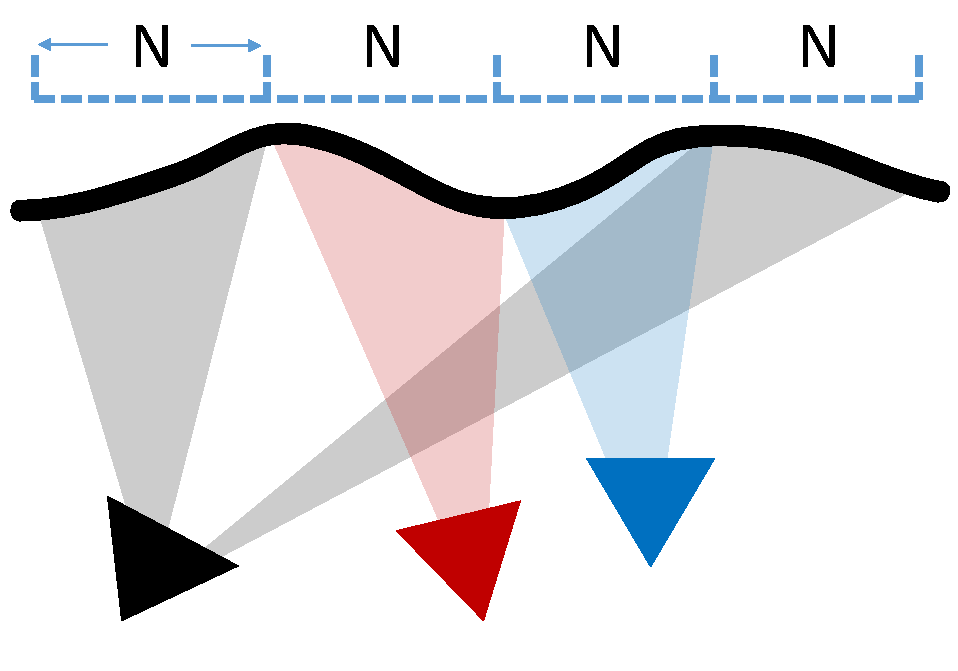
\includegraphics[width=0.48\linewidth]{chapter5/resource/cn_frame_distribution_cropped.pdf}
\label{fig:frameDist}
}
\subfloat[System condition]{
\centering
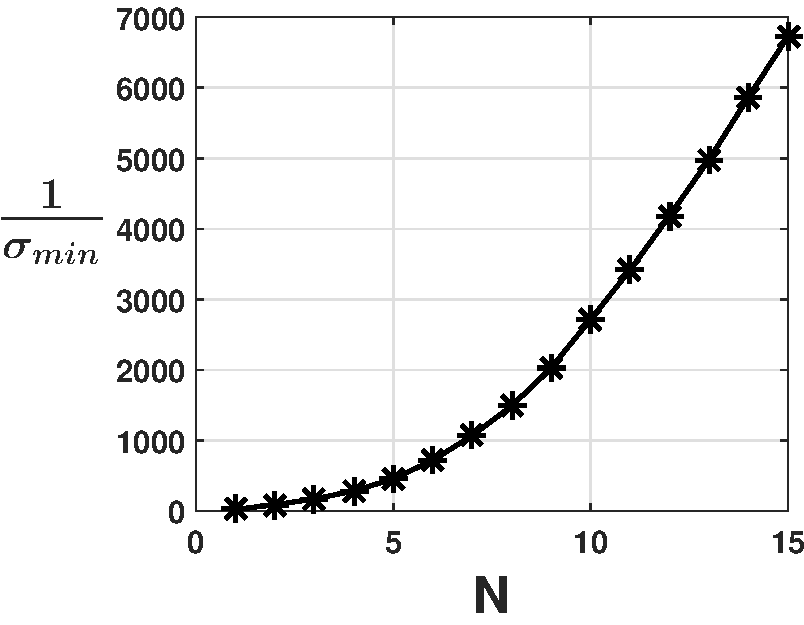
\includegraphics[width=0.43\linewidth]{chapter5/resource/cn.pdf}
\label{fig:frameDist_cond}
}
\caption{The reconstructability of the system is lower if the period of single-camera capture is longer.}
\end{figure}

In our experiment, we observe the reconstructability is closely related to the camera motion and the object motion. 
Specifically, if shape $\mathbf{S}_j$ is the most related shape to $\mathbf{S}_f$, as indicated by $\allT$, the relative directions of viewing rays $\mathbf{r}_f$ and $\mathbf{r}_j$, which are associated with shape $\mathbf{S}_f$ and $\mathbf{S}_j$ respectively (note we only have one point per shape in this analysis), determine the reconstructability. If the directions of $\mathbf{r}_f$ and $\mathbf{r}_j$ converge, \ie the camera motion is relatively larger than the object motion, the reconstructability is higher. Otherwise, it is lower. 
In the case of one handheld camera, the camera motion is much smaller than the dynamic objects,  and the viewing rays diverge, so the reconstructability is low. In contrast, if $\mathbf{r}_j$ and $\mathbf{r}_f$ are associated with different video cameras, the distance between the camera centers is much larger than the motion of the object. Hence the reconstructability is high.
This observation is analogous to the classic triangulation of static scenes, where small baselines produce inaccurate reconstruction. Note the same conclusion was also made by Park \etal~\cite{park20153d}, though their reconstruction algorithm is different from ours.



\subsection{Shape Approximation Residual} \label{sec:shape_approximation}
While $\mathbf{A}$ depends on the viewing ray directions, which are available before reconstruction, $\mathbf{b}$ relies on the actual unknown positions of the ground truth structure $\allX^*$. To achieve accurate reconstruction, each value in the vector $\mathbf{b}$ should be close to 0. 

\begin{figure}
\centering
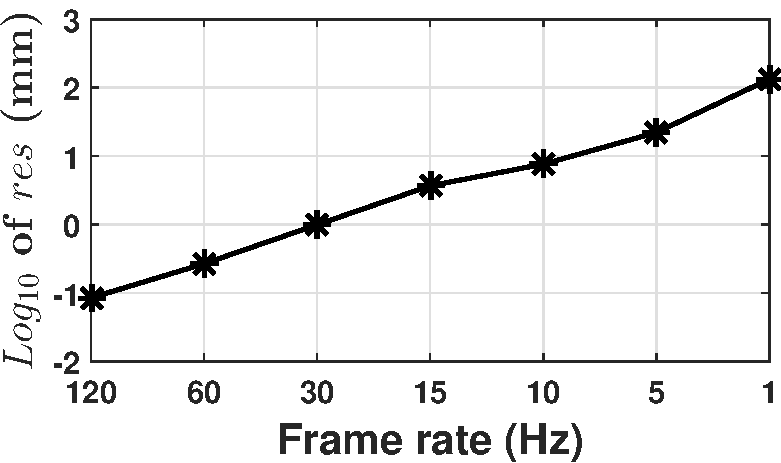
\includegraphics[width=0.80\textwidth]{chapter5/resource/residual.pdf}
\caption{Average residual $res$ (over 130 motion capture datasets present in \cite{cg-2007-2}) at different camera frame rates.}
\label{fig:residual}
\end{figure}

Since in Equation (\ref{eq:b}), $(I-\allT)_{:f}^\text{T}$ is sparse. $\mathbf{b}_f$ can be considered as a linear combination of a few columns of matrix $\allX^*(I-\allT)$, and then dot product with the unit vector $\mathbf{r}_f$.
Therefore, the value of $\mathbf{b}_f$ mainly relies on $||\allX^*(I-\allT)||_\text{F}$.
Accordingly, we define the residual per point as
\begin{equation}
res = \frac{1}{PF}||\allX^*(I-\allT)||_\text{F}. \label{eq:residual}
\end{equation}
The residual $res$ is small if all the shapes can be well represented by other shapes. It relies on speed of object motion and the capturing frame rate. 
We test the residual $res$ given motion capture data sampled at different frame rates. Figure \ref{fig:residual} shows $res$ becomes larger as the frame rate goes down. This fits the intuition that shapes that are tempo-spatially farther away are less correlated. This also implies that our method cannot achieve accurate reconstruction from discrete images with large temporal discrepancy. 


\subsection{Importance of Image Sequencing} \label{sec:importance_of_image_sequencing}
The temporal order of images, \ie image sequencing, plays an important role in dynamic object reconstruction \cite{Park_ECCV2010,zheng2014joint,Valmadre_CVPR2012}. The work by \cite{Valmadre_CVPR2012} generalizes the method by \cite{Park_ECCV2010} in a new framework based on high-pass filters. Here, we briefly describe the method by \citet{Valmadre_CVPR2012} and its relation to our method, from which it can be revealed why their methods require sequencing information as opposed to ours. 

Assuming the object moves smoothly in the space, Valmadre \etal~\cite{Valmadre_CVPR2012} triangulate the 3D trajectory of an 3D point by minimizing its response to a set of high-pass filters.
Given a predefined high pass filter $g=[g_M,\dots,g_1]$, the trajectory is estimated by 
\begin{equation}
\underset{\allX}{\text{minimize}} ~ || \allX G||_\text{F}^2,
\label{eq:valmadre_equ}
\end{equation}
where $G$ is defined as
\begin{equation}
G = \left[ 
\begin{matrix}
g_M  	&  		 &   	  	\\
\vdots	& \ddots &    	  	\\
g_1		& \ddots & g_M	  	\\
		& \ddots & \ddots 	\\
		&		 & g_1	
\end{matrix}
\right]
\label{eq:valmadre_filter_G}
\end{equation}
Each column of $G$ is a high-pass filter for the local region of a trajectory. From the formulation, it is required all the shapes (columns of $\allX$) should be ordered temporally. 

By comparing Equation (\ref{eq:valmadre_equ}) with Equation (\ref{eq:recon_original}), it can be shown $G$ is equivalent to our method with a predefined value of $\allT$, under the assumption that all the columns of $\allX$ are ordered in temporal order. 
For instance,  if the high pass filter is set to $g=[1,-1]$, it is equivalent (ignoring the difference at boundary) that $\allT$ is set to
\begin{equation}
\allT = \left[
\begin{matrix}
0 &   & \\
1 & 0 & \\[-7pt]
  &	1 & \ddots \\[-7pt]
  &   & \ddots 
\end{matrix}.
\right]
\end{equation}
Therefore, an alternative interpretation of their method \cite{Valmadre_CVPR2012} using the high-pass filter $g=[1,-1]$ in terms of our theory is approximating the current shape by the temporally closest shape. 

Another high-pass filter proposed by \citet{Valmadre_CVPR2012} is $[-1, 2, -1]$, which in our case is equivalent to fixing the weights of two neighboring shapes to 0.5. %as follows
%\begin{equation}
%\allT = \left[
%\begin{matrix}	  
%	0.5   &      & \\
%	0   & 0.5  & \\[-7pt]
%	0.5 & 0    & \ddots \\[-7pt]
% 	    & 0.5  & \ddots \\[-7pt]
%  		&      & \ddots 
%\end{matrix}
%\right]
%\end{equation}
In effect, their method can be deemed as our method with predefined $\allT$. 

The importance of sequencing can be further revealed from analysis of residual defined by Equation (\ref{eq:residual}). The residual will be large if columns of $\allX^*$ are randomly shuffled. In contrast, our method cleverly and automatically picks the most related shapes (matrix columns) using compressive sensing to produce small $res$.


%%%%%%%%%%%%%%%%%%%%%%%%%%%%%%%%%%%%%%%%%%%%%%%%%%%%%%%%%%%%%%%%%%%%%%%%%%%%%%%%

%%%%%%%%%%%%%%%%%%%%%%%%%%%%%%%%%%%%%%%%%%%%%%%%%%%%%%%%%%%%%%%%%%%%%%%%%%%%%%%% 


\section{Experiments} \label{sec:experiment}
In our experiments, we evaluate our algorithm on both synthetic and real datasets. $\lambda_1$ and $\lambda_2$ in Equation (\ref{eq:ourproblem_final}) are set empirically to 0.05 and 0.1 for all the experiments. To alleviate the influence of different camera system scales (\ie~differing the scale of $\allX$), the average distance between camera centers is normalized to 1 before applying our method. The soft constraint parameterization is used only in the presence of noisy measurements.

\subsection{Simulation}
We use synthetic datasets to evaluate the accuracy and robustness of our methods, and also compare with two state-of-the-art methods.
To generate synthetic data, we use the real motion capture datasets in the work by \citet{cg-2007-2}, and leverage them as ground truth structure for our estimation.
The whole datasets contain 130 different real motions including hopping, jogging, cartwheel, punching, \emph{etc}.
Each motion capture dataset is comprised of the temporal sequences of a common set of 44 3D points in real scale, which corresponds within our framework to ground truth structure $\allX_{GT}$. The frame rate of the motion datasets, \ie~the sampling rate of real continuous motion, is 120 Hz. The length of each dataset ranges from 45 to 701 frames, and with an average of 273 frames. 

These 3D points are projected onto virtual cameras to generate input 2D measures into our methods.
We select 4 virtual cameras with a resolution of 1M and focal length of 1000, and we position the static cameras around the centroid defined by $\allX_{GT}$. 
The distance of the camera to the centroid is approximately twice the scale of $\allX_{GT}$, and on average the distance is 2.7 meters.
Considering the frame rate of the motion capture datasets is 120 Hz and there are 4 virtual cameras, the average frame rate for each camera is 30 Hz.
%The ratio between the distance to the centroid and the maximal distance between any two points in $\allX_{GT}$ is set to one.
Every temporal 3D capture is randomly assigned to each camera to build 4 disjoint image sequences. %To better evaluate how well our method recover the coefficient matrix $\allT$, 
Unless otherwise mentioned, we enforce that no temporally consecutive captures are assigned to the same image sequence.

To evaluate our method, the Euclidean errors between the ground truth and estimated 3D points are computed.
We define the accuracy by counting the percentage of points having errors less than thresholds of $10$, $20$, $30$, $40$, $50$, and $100$ mm.

\subsubsection{Accuracy} \label{sec:experiment_accuracy}
\begin{figure}
\centering
  \begin{minipage}[c]{0.8\linewidth}
    \centering
    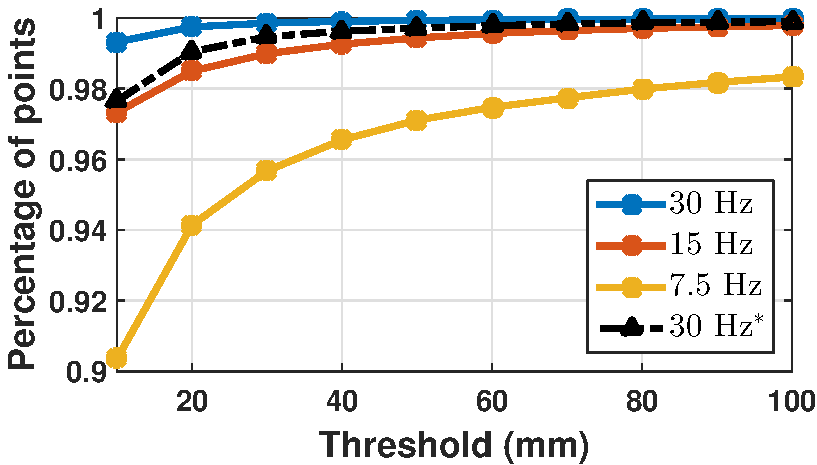
\includegraphics[width=1\linewidth]{chapter5/resource/error_at_diff_framerate.pdf}  
  \end{minipage} \\
\centering
  \begin{minipage}[c]{1\linewidth}
    \centering
 \begin{tabular}[b]{|c|*{6}{c|}}
	\hline
  \backslashbox{Frame rate\kern-1em}{\kern-1emThreshold}
	& {10} & {20} & {30} & {40} & {50} & {100}\\\hline
	{30}  & 0.9933 &   0.9975  &  0.9986  &  0.9991  &  0.9994  &  0.9998\\
	\hline
	{15}  &  0.9734  &  0.9850  &  0.9899  &  0.9926 &   0.9944  &  0.9979\\
	\hline
	{7.5}  &  0.9036  &  0.9415  &  0.9568 &   0.9655 &   0.9711 &  0.9833\\
	\hline	
	\hline
	\begin{tabular}{@{}c@{}} 30 (unconstrained \\ assignment) \end{tabular} & 0.9766  &  0.9905 &   0.9947 &   0.9963  &  0.9971 &   0.9990\\
	\hline	
  \end{tabular}
\end{minipage}
\caption{The reconstruction accuracy given different camera frame rates. We also test the case that the captures of object motion are randomly assigned to any of the image sequences without any constraint. 30 Hz$^*$ in the figure represents the unconstrained assignment.}
\label{fig:error_framerate}
\end{figure}

\begin{figure}
\centering
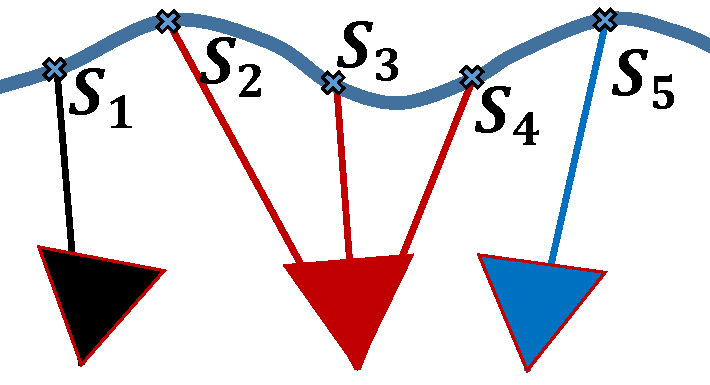
\includegraphics[width=0.65\textwidth]{chapter5/resource/unconstrained_assignment_cropped.pdf}
\caption{Consecutive captures are assigned to the same red camera. For easy visualizations, only one point per shape is drawn.}
\label{fig:unconstrained_assign}
\end{figure}

\textbf{Different frame rates.}
We first evaluate how the algorithm behaves under different frame rates of capturing.
2D measures without noise are used to evaluate the accuracy of our method. In addition to the original motion capture data at 120 Hz, we also downsample the data to 60 and 30 Hz, so that each camera has frame rate of 15 and 7.5 Hz on average. As shown in Figure \ref{fig:error_framerate}, the accuracy becomes worse as the frame rate gets slower. 
The main reason is that the self-representation residual is larger at lower frame rate. We notice that at a frame rate of 7.5 Hz, our method does not work well on the quick motions with large and nonlinear shape deformation, such as hopping or arms rotation. However, still  more than 97\% of 3D points have errors less than 5 cm, which is already very small considering the scale of a person and the distance range of the cameras.
%One of the main reasons is that the residual becomes larger and then the reconstructability becomes smaller. Note that the residual depends on both the frame rate and the speed of motion.
%We also notice that \hl{to be continued...}
%which is already very small considering the scale of the person and the distance of cameras from the person.

\textbf{Local temporal information.}
We also quantitatively evaluate the estimated $\allT$. Using the same two measures described in Section \ref{sec:principle}, 
we get values of 0.9902 and 0.9923, compared to 0.9972 and 0.9994 if the 3D points are given. Therefore, our method very accurately recovers the local temporal information.

\textbf{Unconstrained capture assignment}
We test the case that each capture is randomly assigned to one of the four cameras so that temporally consecutive captures could have a chance to be assigned to the same camera, as is shown in Figure \ref{fig:unconstrained_assign}. In this specific case, shapes $\mathbf{S}_1$ and $\mathbf{S}_5$ are used to represent $\mathbf{S}_2$, $\mathbf{S}_3$ and $\mathbf{S}_4$. Based on theory in Section \ref{sec:shape_approximation}, using spatially farther away shapes to represent the current shape has larger residual and hence larger reconstruction errors, as is validated in Figure \ref{fig:error_framerate}.
 
\subsubsection{Corrupted Measurements}

\begin{figure*}
\centering
  \begin{minipage}[c]{0.8\linewidth}
    \centering
    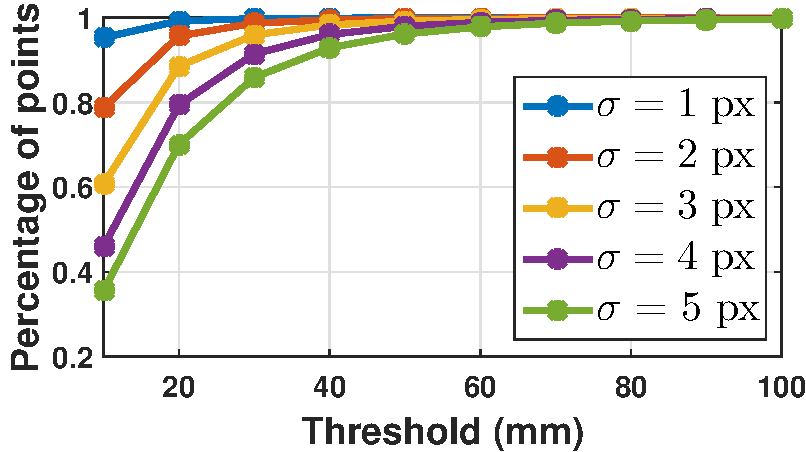
\includegraphics[width=1\linewidth]{chapter5/resource/noise_measure_plot.pdf}  
  \end{minipage} \\
\centering  
  \begin{minipage}[c]{0.8\linewidth}
    \centering
 \begin{tabular}[b]{|c|*{6}{c|}}
	\hline
  \backslashbox{Noise\kern-3em}{\kern-1emThreshold}
	& {10} & {20} & {30} & {40} & {50} & {100}\\\hline
	{$\mathcal{N}(0,1)$}  & 0.9529  &  0.9925 &   0.9974  &  0.9987  &  0.9992 &   0.9998\\
	\hline
	{$\mathcal{N}(0,2)$}  &   0.7878 &   0.9568  &  0.9869 &   0.9949 &   0.9976 &   0.9997\\
	\hline
	{$\mathcal{N}(0,3)$}  & 0.6074 &   0.8855 &   0.9593  &  0.9828  &  0.9917  &  0.9991\\
	\hline
	{$\mathcal{N}(0,4)$}  & 0.4601  &  0.7941 &   0.9144  &  0.9602  &  0.9797  &  0.9980\\
	\hline
	{$\mathcal{N}(0,5)$}  &  0.3551  &  0.7008  &  0.8590  &  0.9287 &   0.9615  &  0.9966\\
	\hline	
\end{tabular}
\end{minipage}
\caption{The reconstruction accuracy when the 2D observations are corrupted with Gaussian noise of different standard deviation ($\sigma$).}
\label{fig:error_noise}
\end{figure*}
\begin{figure}[t]
\centering
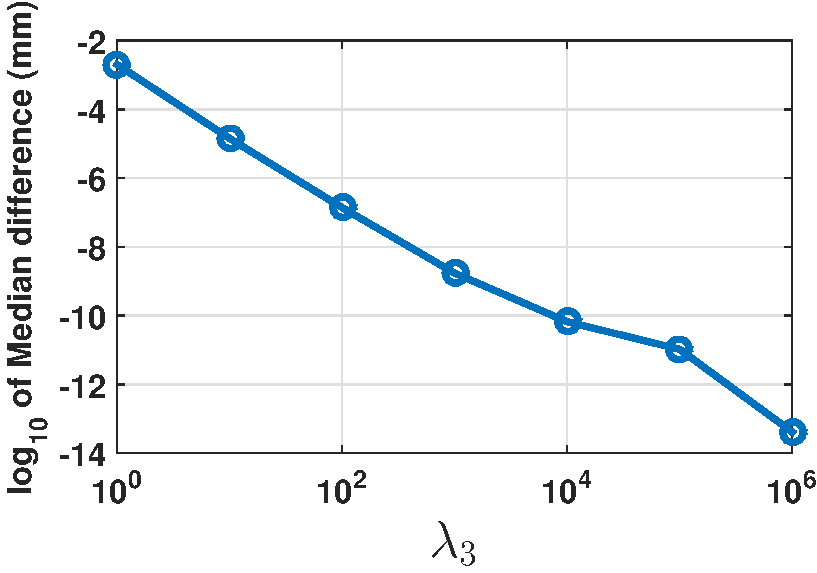
\includegraphics[width=0.75\textwidth]{chapter5/resource/different_lambda.pdf}
\caption{The difference of the estimated results by the hard constraint formulation in Equation (\ref{eq:X_representedBy_d_all}) and the soft constraint formulation in Equation (\ref{eq:soft_constraint}) with different $\lambda_3$} 
\label{fig:soft_hard_diff}
\end{figure}

To evaluate the robustness of our method, we test it in the case of noisy measurements and missing data.

\textbf{Noisy measurements.} We add zero-mean Gaussian noise with different standard deviations to the 2D measures. Considering that the focal length of the image is 1000 pixel, one pixel error corresponds to one millimeter if the object is one meter away.
We apply the soft constraint formulation described in Section \ref{sec:noisy_measure} and empirically set the parameter $\lambda_3$ to 100. As depicted in Figure \ref{fig:error_noise}, the quality of reconstruction degrades as the noise level increases. As $\lambda_3$ increases, the soft constraint is more close to the hard constraint. % since more penalty is posed if the estimated points are away from the viewing ray. 
We evaluate the difference of the estimated results by the hard constraint formulation and the soft constraint formulation with different $\lambda_3$, and we show the median difference in Figure \ref{fig:soft_hard_diff}. It is apparent that as $\lambda_3$ increases, the difference of the output between the two formulations becomes smaller.

We have tested the hard constraint formulation using noisy measurements, and the overall accuracy of the output is very similar. Though the soft constraint appears more robust in the presence of noise as it allows the points off the viewing ray, there is no guarantee or proof this constraint will achieve more accurate results, as it depends on the exact motion of the objects.


\textbf{Missing data.} %Missing observations occur in practice due to occlusion or mis-detection. 
In our evaluation, we randomly set some 2D measures to be unavailable. Figure \ref{fig:error_occlusion} depicts the accuracy under different percentages of missing data. We observe that under 20\% of occlusion there is not much difference in reconstruction accuracy. Moreover, under a large amount of 40\% occlusion, our method still produces accurate results,  with 94.38\% of points having errors less than 30 mm. 

Our method essentially linearly interpolates the 3D points along the trajectory using estimated  $\allT$. It can still produce 3D estimates in the presence of consecutive missing observations across time, but the accuracy in such scenarios depends on the object motion. Particularly, given large displacement of nonlinear motion, our method is likely to produce less accurate results.

\begin{figure*}
\centering
  \begin{minipage}[c]{0.8\linewidth}
    \centering
    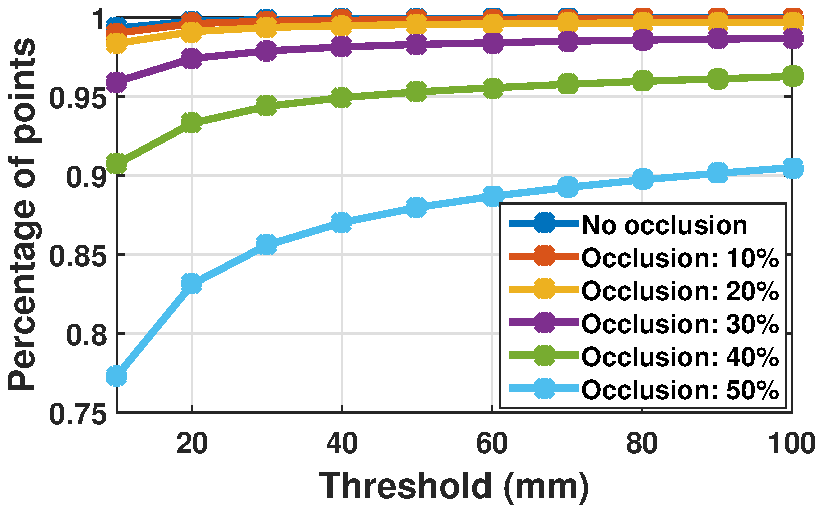
\includegraphics[width=1\linewidth]{chapter5/resource/occlusion_measure_plot.pdf}  
  \end{minipage} \\
  \begin{minipage}[c]{0.8\linewidth}
    \centering
\begin{tabular}[b]{|c|*{6}{c|}}
	\hline
  \backslashbox{Miss rate\kern-2em}{\kern-1emThreshold}
	& {10} &{20} & {30} & {40} & {50} & {100} \\\hline
	{0\%} & 0.9933 & 0.9975 & 0.9986 & 0.9991 & 0.9994 & 0.9998 \\
	\hline
	{10\%} & 0.9901 & 0.9961 & 0.9975  &  0.9982  &  0.9986  &  0.9993 \\
	\hline
	{20\%} & 0.9835  &  0.9910 &   0.9936 &   0.9948  &  0.9955 &   0.9968 \\
	\hline
	{30\%} & 0.9594  &  0.9740  &  0.9788 &   0.9813 &   0.9829 &   0.9868 \\
	\hline
	{40\%} & 0.9074  &  0.9331  &  0.9438  &  0.9493 &   0.9529 &   0.9626 \\
	\hline
	{50\%} & 0.7734  &  0.8313  &  0.8560  &  0.8703 &   0.8798 &   0.9050 \\
	\hline
\end{tabular}
\end{minipage}
\caption{The reconstruction accuracy under different percentages of occluded points.}
\label{fig:error_occlusion}
\end{figure*}

%and use the same evaluation criterion as described in Sec.~\ref{sec:experiment_accuracy}. 
%Figs.~\ref{fig:hard_constraint_noise} and \ref{fig:soft_constraint_noise} show the errors of our method using hard and soft constraint for the parameterization of $\allX$. 
 
%\begin{figure}[t]
%\centering
%\includegraphics[width=0.4\textwidth]{resource/initialization/Init_result_compare.pdf}
%\caption{The average Euclidean error of the initialization and the final output.}
%\label{fig:initialization_optimal_noise}
%\end{figure}

 
\subsubsection{Comparison to Other Methods}
We compare our method with one of the non-rigid structure from motion methods \cite{dai2014simple} and one of the trajectory triangulation methods \cite{Valmadre_CVPR2012}. Both of these methods are state-of-the-art for dynamic object reconstruction.

\textbf{NRSFM method.} Non-rigid structure from motion (NRSFM) recovers both the camera motion and the dynamic structure. It is tempting to use those methods to solve our problem, since our problem with known camera poses seems to be easier. 
However, most NRSFM methods work on an orthographic or weak perspective camera model, and it is unclear of their applicability under the perspective model. \citet{Park_ECCV2010} test the NRSFM methods by \citet{Akhter_NIPS08,torresani2008nonrigid,paladini2009factorization} under a perspective camera model, but all of them fail to produce reasonably good results. In this paper, we test the state-of-the-art NRSFM method by \citet{dai2014simple}.

%The first method we compare to is prior-free NRSFM By Dai \etal \cite{dai2014simple}.
The method by \citet{dai2014simple} is based on the assumption that each non-rigid shape $\oneX_f$ is a linear combination of $K$ shape bases, and hence the shape matrix (corresponding to $\allX$ in our problem description) has low rank.
After estimating the camera motion,  they recover the structure by minimizing the rank of the shape matrix, which is achieved through the minimization of the matrix nuclear norm.  Their method applies to an orthographic camera model, but can be easily adapted to a perspective model, as described below. 

We use the block matrix method proposed in the work by \citet{dai2014simple}. Denoting
\begin{equation}
\allX^\# = 
\begin{bmatrix}
X_{(1,1)}& \dots& X_{(P,1)} & Y_{(1,1)}& \dots& Y_{(P,F)} & Z_{(1,1)}& \dots& Z_{(P,F)} \\
\vdots   &  				& \vdots   & \vdots 		  & \vdots   & \vdots			  \\
X_{(1,F)}& \dots& X_{(P,F)} & Y_{(1,F)}& \dots& Y_{(P,F)} & Z_{(1,1)}& \dots& Z_{(P,F)}\nonumber		  
\end{bmatrix},
\end{equation}
where $\mathbf{X}_{(p,f)} = (X_{(p,f)},Y_{(p,f)},Z_{(p,f)})$, the shape of the object can be recovered through 
\begin{equation}
\begin{aligned}
& \underset{\allX^\#, \allT}{\text{minimize}} &&
||\allX^\#||_* + \mu ||\mathbf{1}_{P\text{x}1} \otimes \allC + (\mathbbm{d} \otimes \mathbf{1}_{3\text{x}1}) \odot \allr - \allX||_{\text{F}}\\
&\text{subject to} && \allX^\# = \mathcal{L}(\allX), \nonumber
\end{aligned}
\end{equation}
where $||\cdot||_*$ is the matrix nuclear norm, $\mu$ is a positive weight, and $\mathcal{L}$ is a linear operator that reshapes $\allX$ into $\allX^\#$. 

This formulation seems attractive at first glance due to its convexity, in contrast to our non-convex formulation. Moreover, their method is shape-based (instead of trajectory-based), and does not require temporal information. 
To test the NRSFM method, We use synthetic data without noise and the random camera configuration shown in Figure \ref{fig:randCam}.
Unfortunately, the qualitative results in Figure \ref{fig:prior_free_Qualitative_result} show that it completely fails, as opposed to our method shown in Figure \ref{fig:ourmethod_Qualitative_result}. 

%The NRSFM method is closely related to our proposed solution. Their method assumes all the shapes can be represented by a linear combination of shape bases, while ours use self-representation. In the typical NRSFM, 

\begin{figure}[]
\centering
\subfloat[Our method accurately reconstructs the 3D points]{
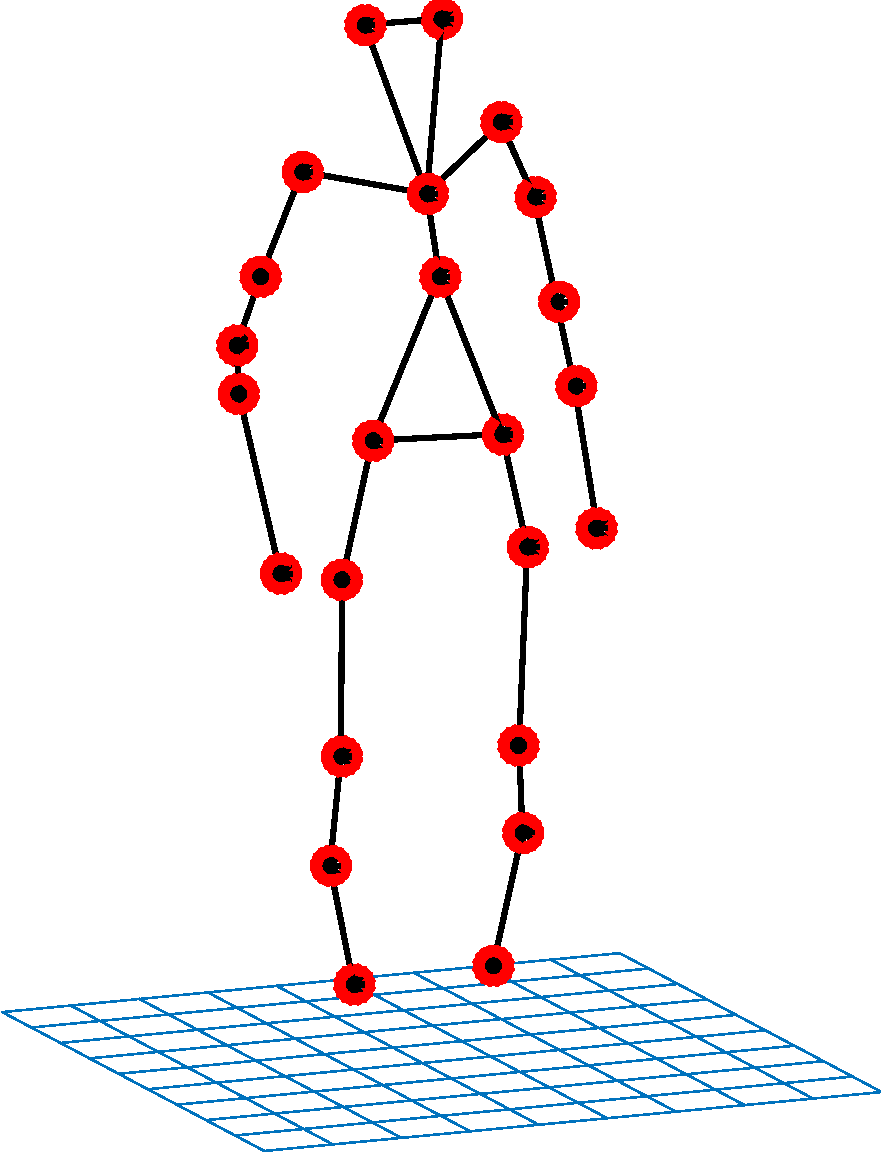
\includegraphics[width=0.155\textwidth]{chapter5/resource/compare_with_prior_free/mymethod/0001.pdf}
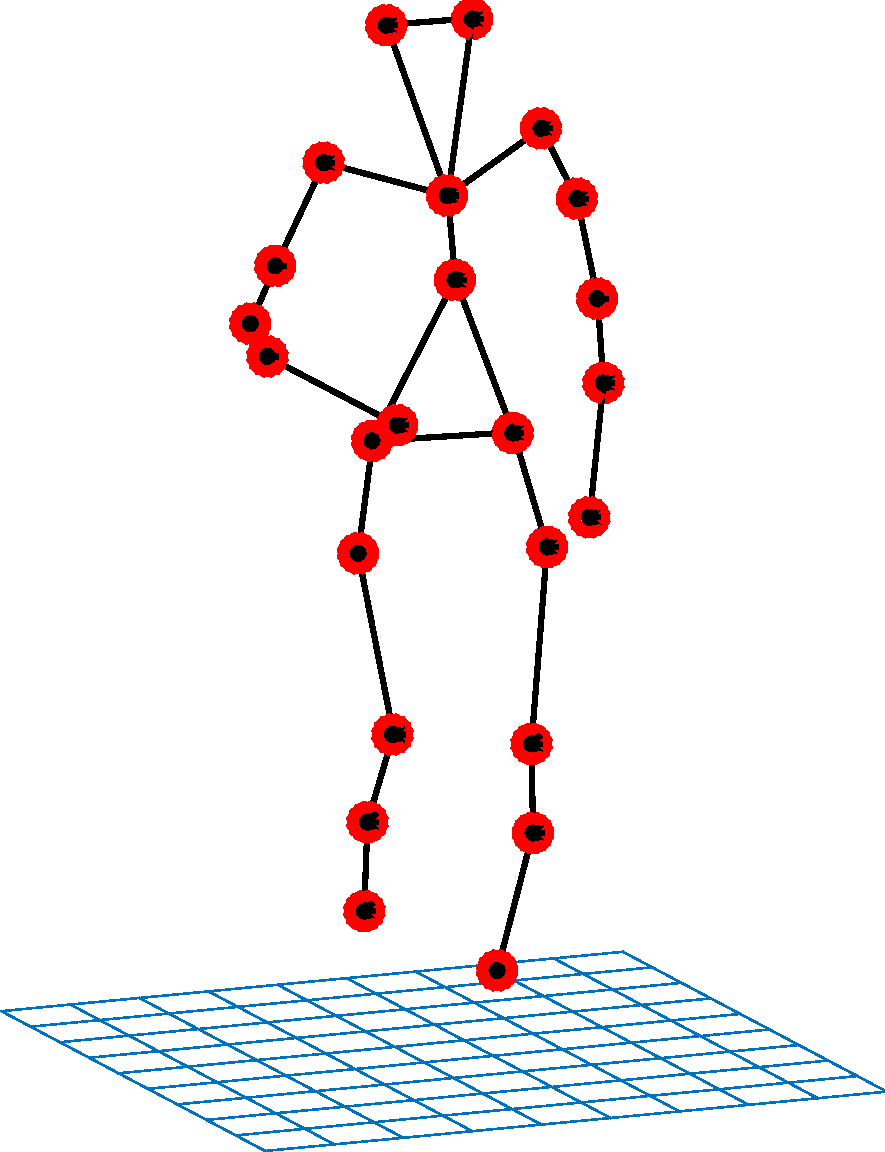
\includegraphics[width=0.155\textwidth]{chapter5/resource/compare_with_prior_free/mymethod/0033.pdf}
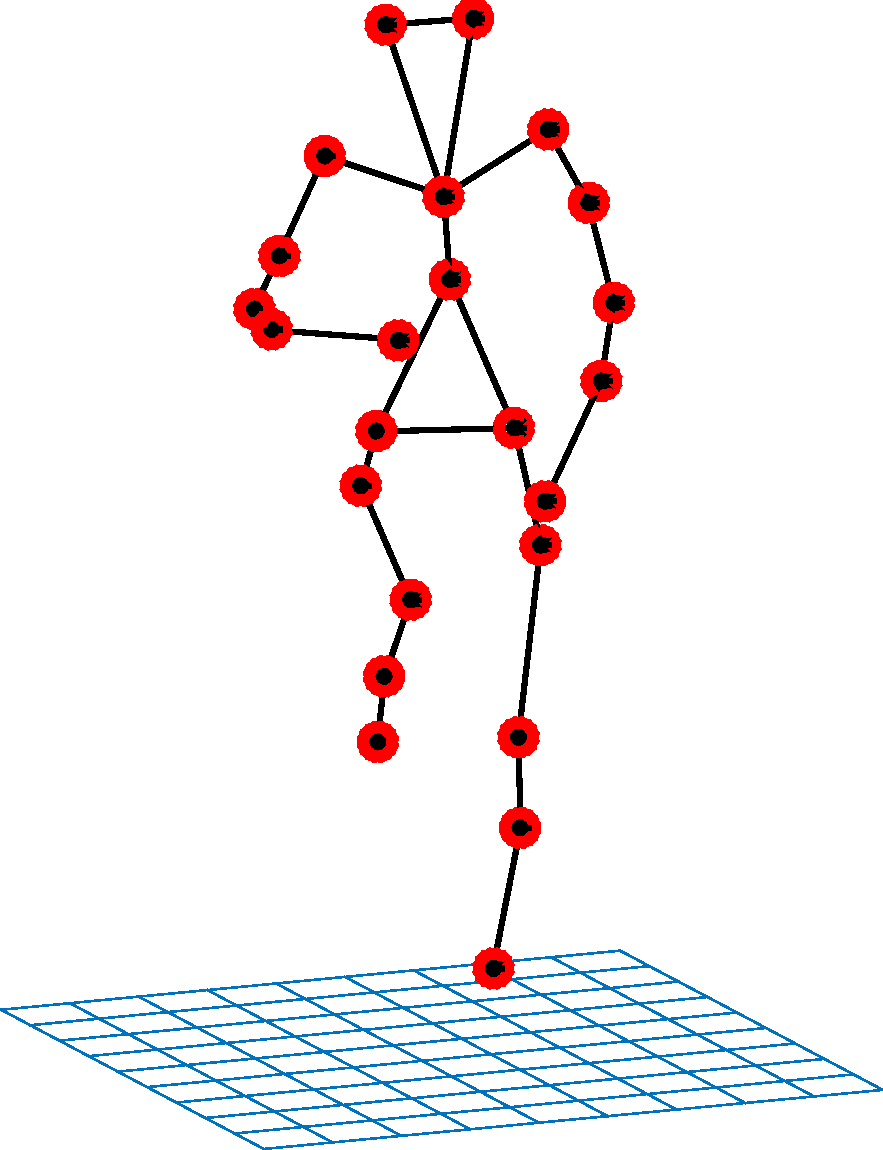
\includegraphics[width=0.155\textwidth]{chapter5/resource/compare_with_prior_free/mymethod/0055.pdf}
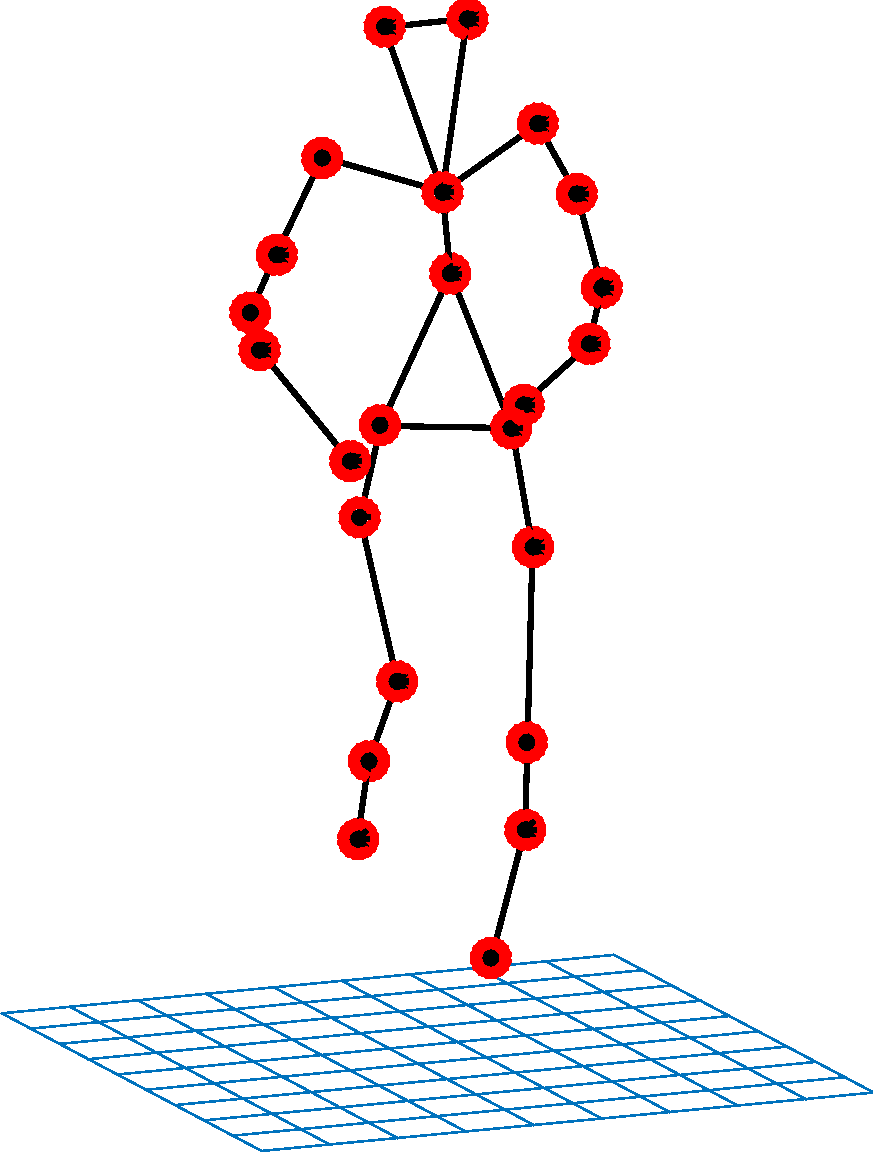
\includegraphics[width=0.155\textwidth]{chapter5/resource/compare_with_prior_free/mymethod/0069.pdf}
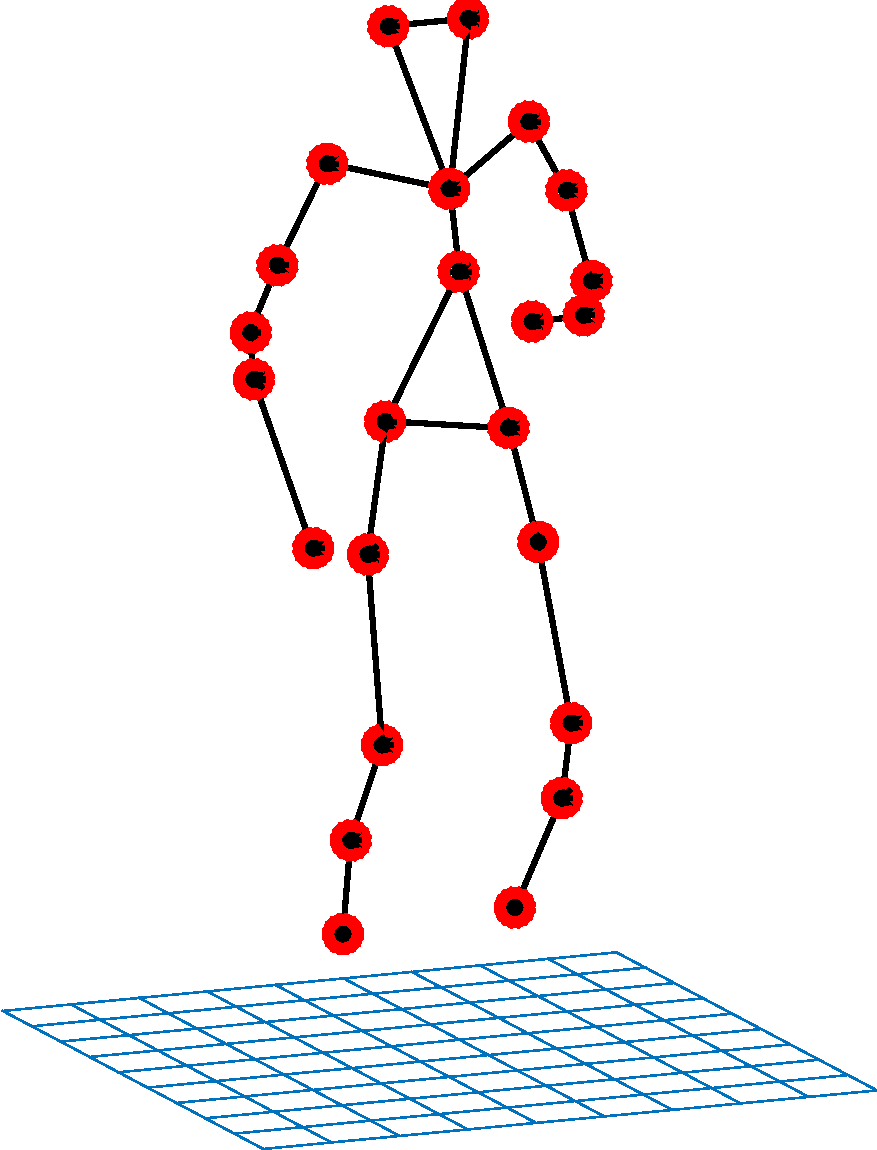
\includegraphics[width=0.155\textwidth]{chapter5/resource/compare_with_prior_free/mymethod/0079.pdf}
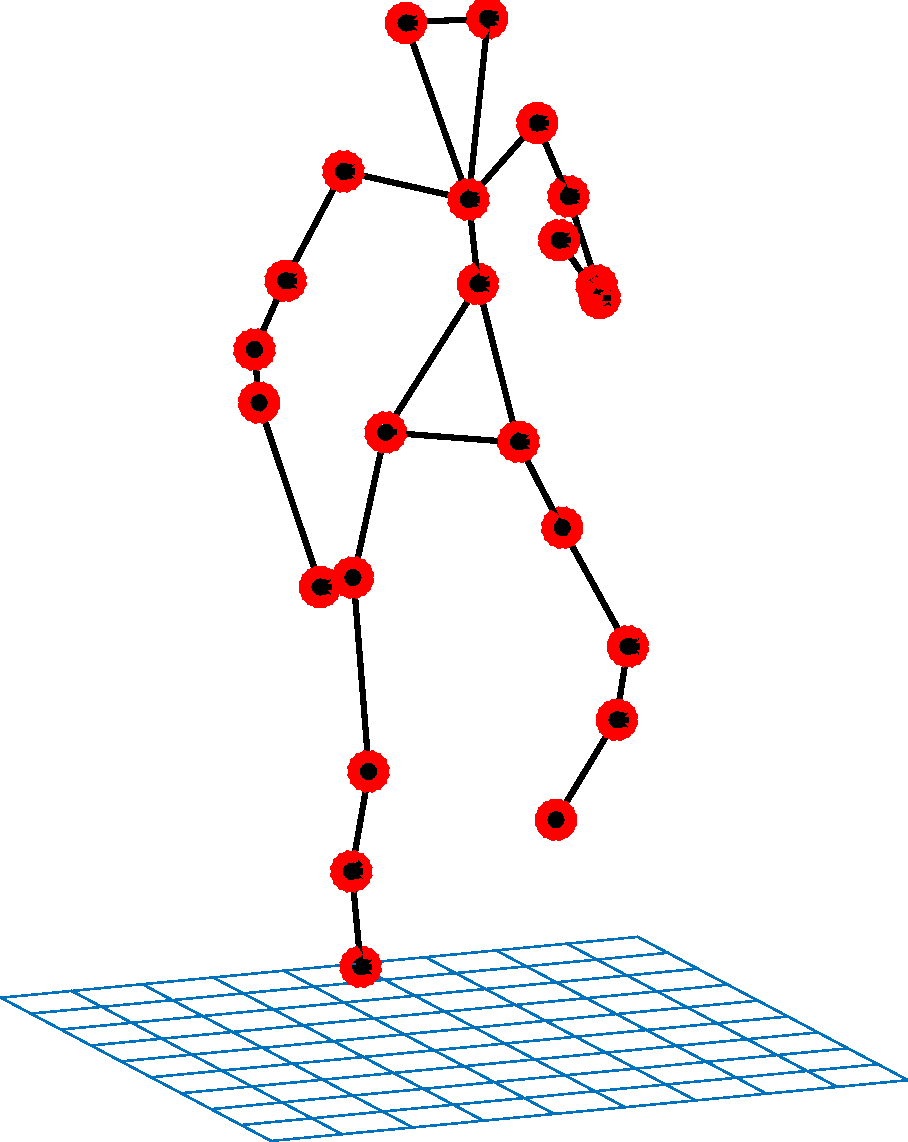
\includegraphics[width=0.155\textwidth]{chapter5/resource/compare_with_prior_free/mymethod/0091.pdf}
\label{fig:ourmethod_Qualitative_result}
}\\
\subfloat[The modified prior-free method \cite{dai2014simple} fails to produce reasonable results]{
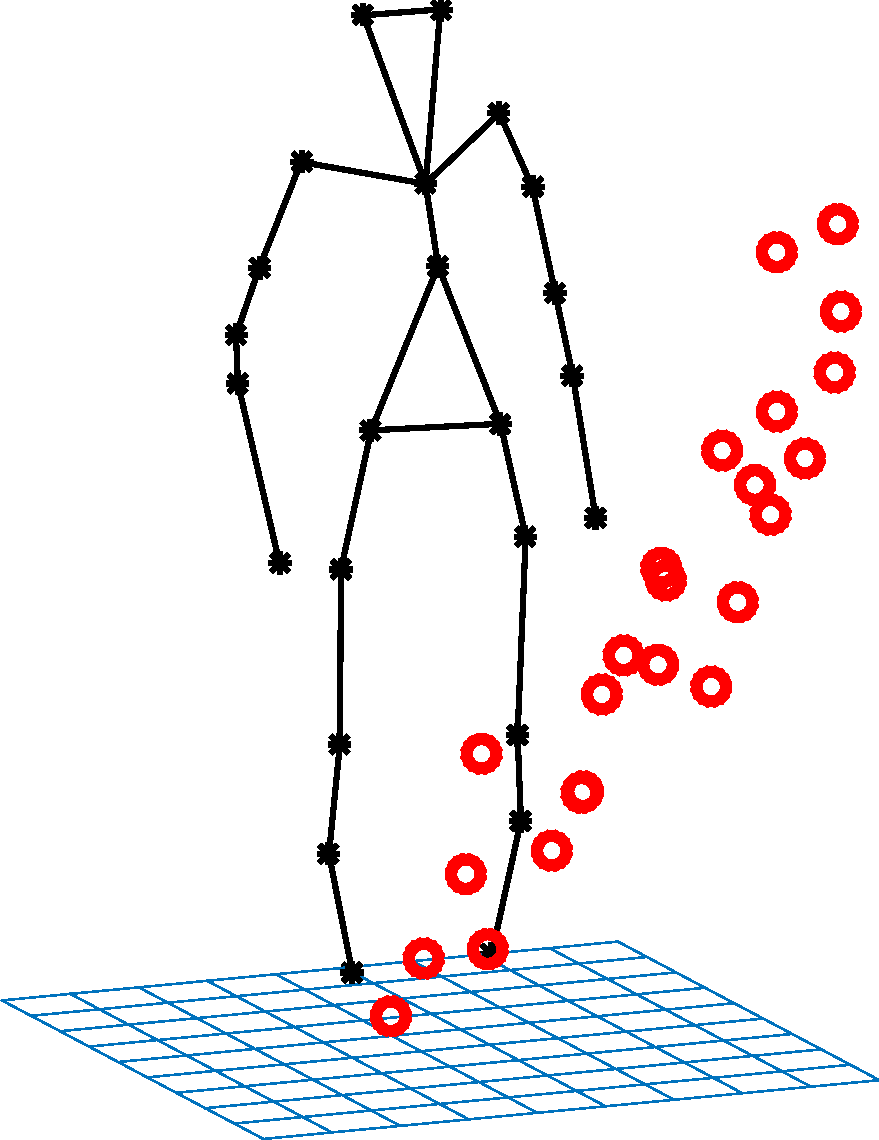
\includegraphics[width=0.155\textwidth]{chapter5/resource/compare_with_prior_free/priorfree/0001.pdf}
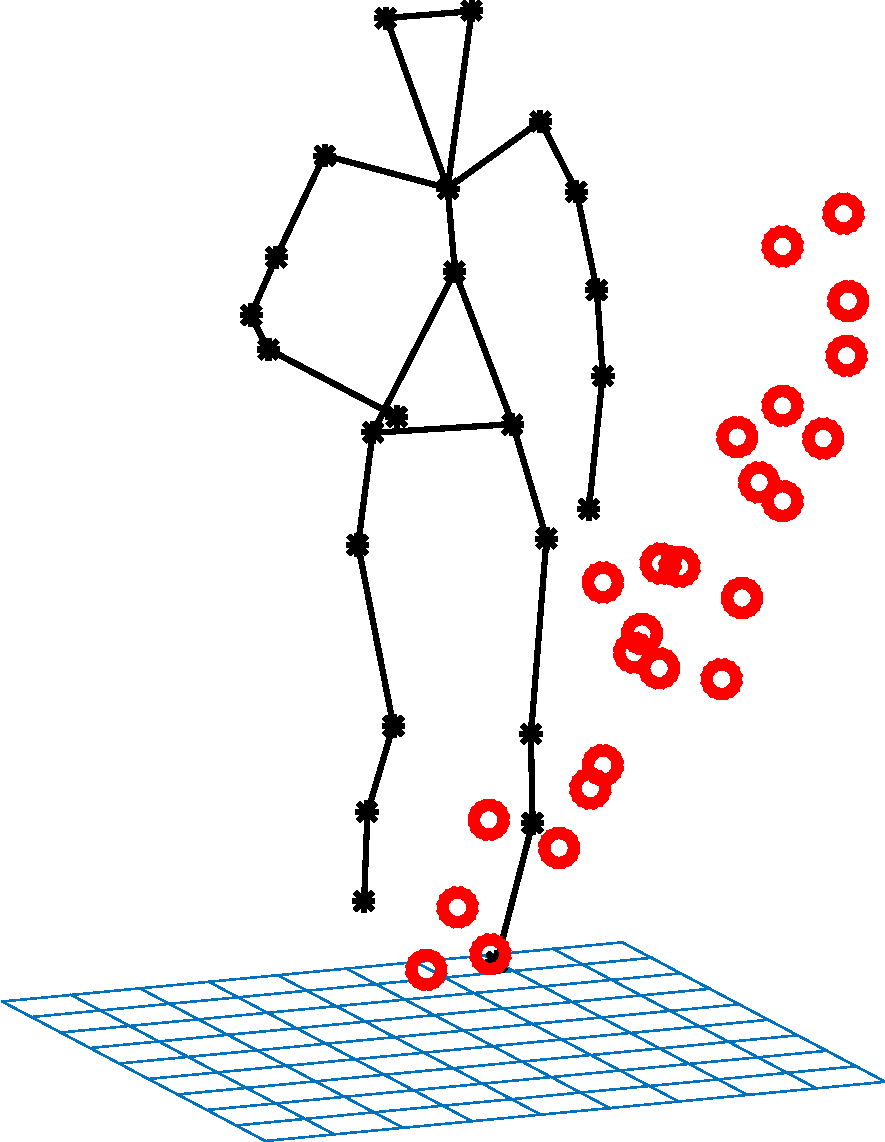
\includegraphics[width=0.155\textwidth]{chapter5/resource/compare_with_prior_free/priorfree/0033.pdf}
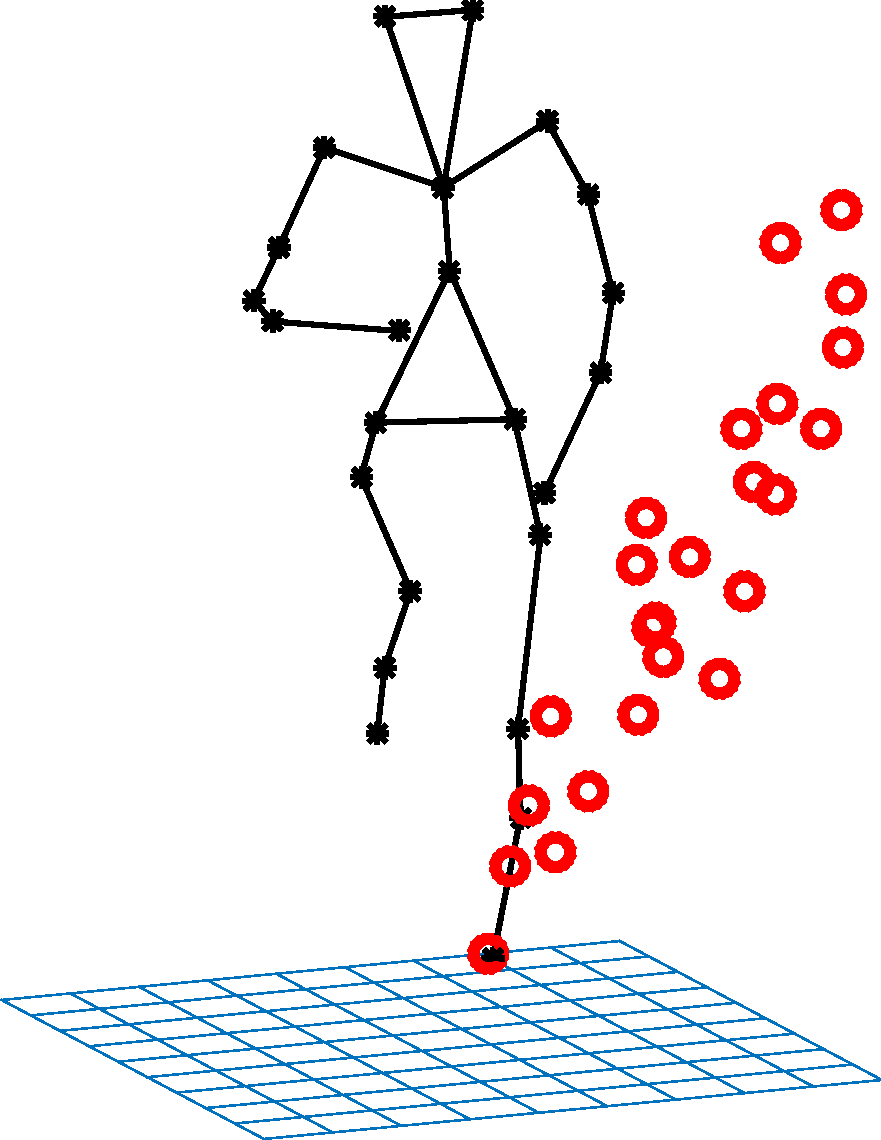
\includegraphics[width=0.155\textwidth]{chapter5/resource/compare_with_prior_free/priorfree/0055.pdf}
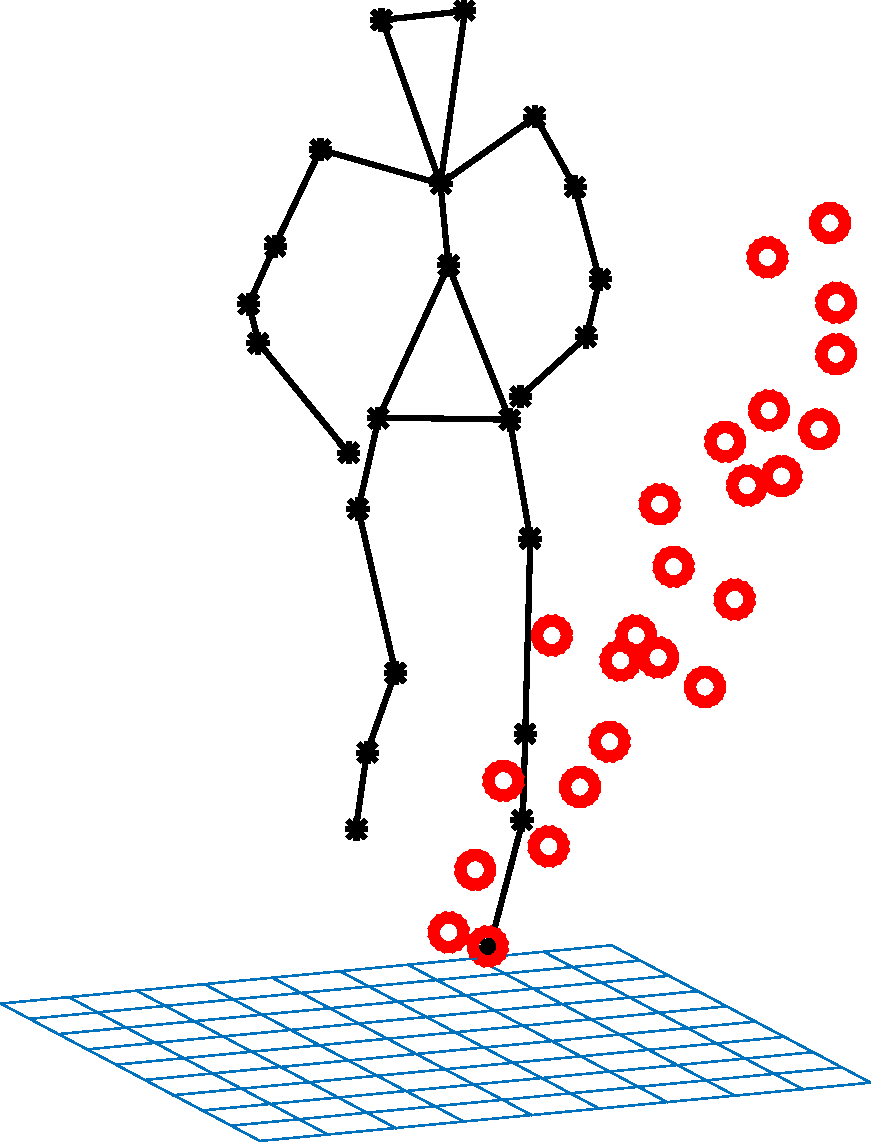
\includegraphics[width=0.155\textwidth]{chapter5/resource/compare_with_prior_free/priorfree/0069.pdf}
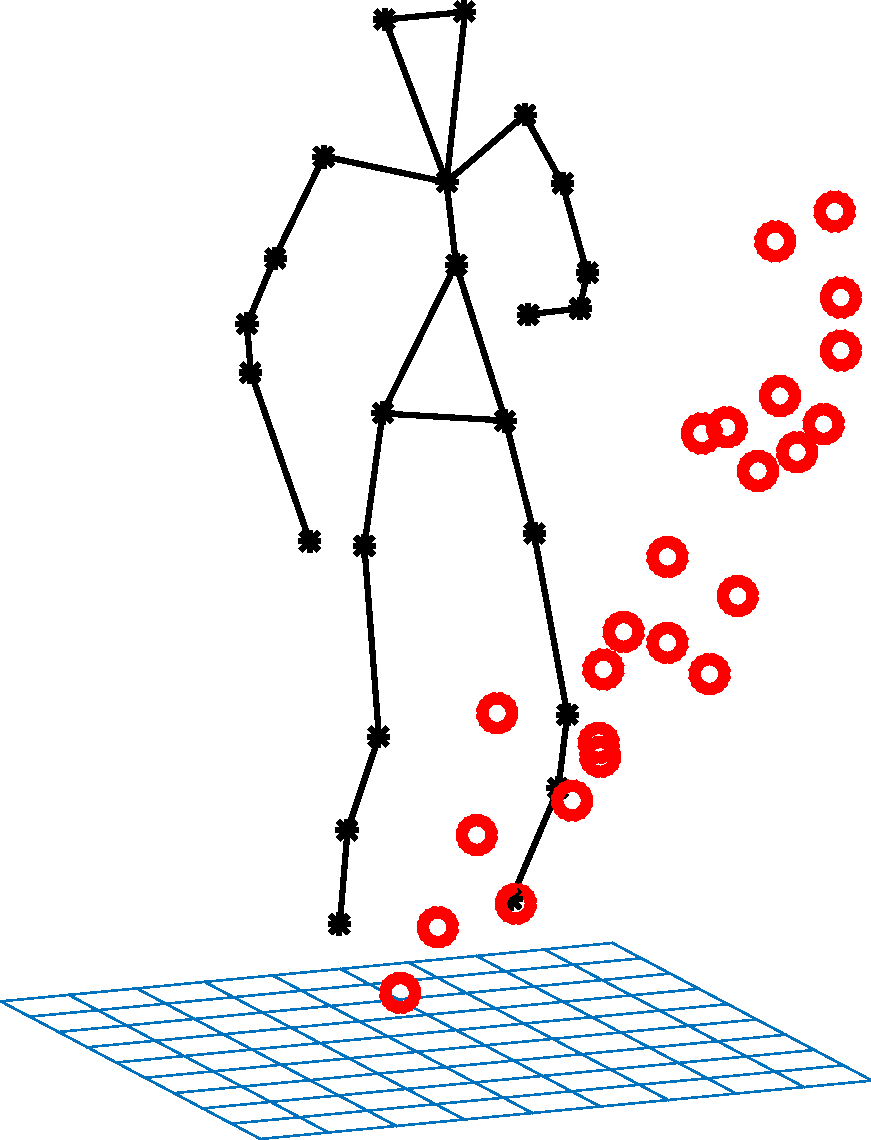
\includegraphics[width=0.155\textwidth]{chapter5/resource/compare_with_prior_free/priorfree/0079.pdf}
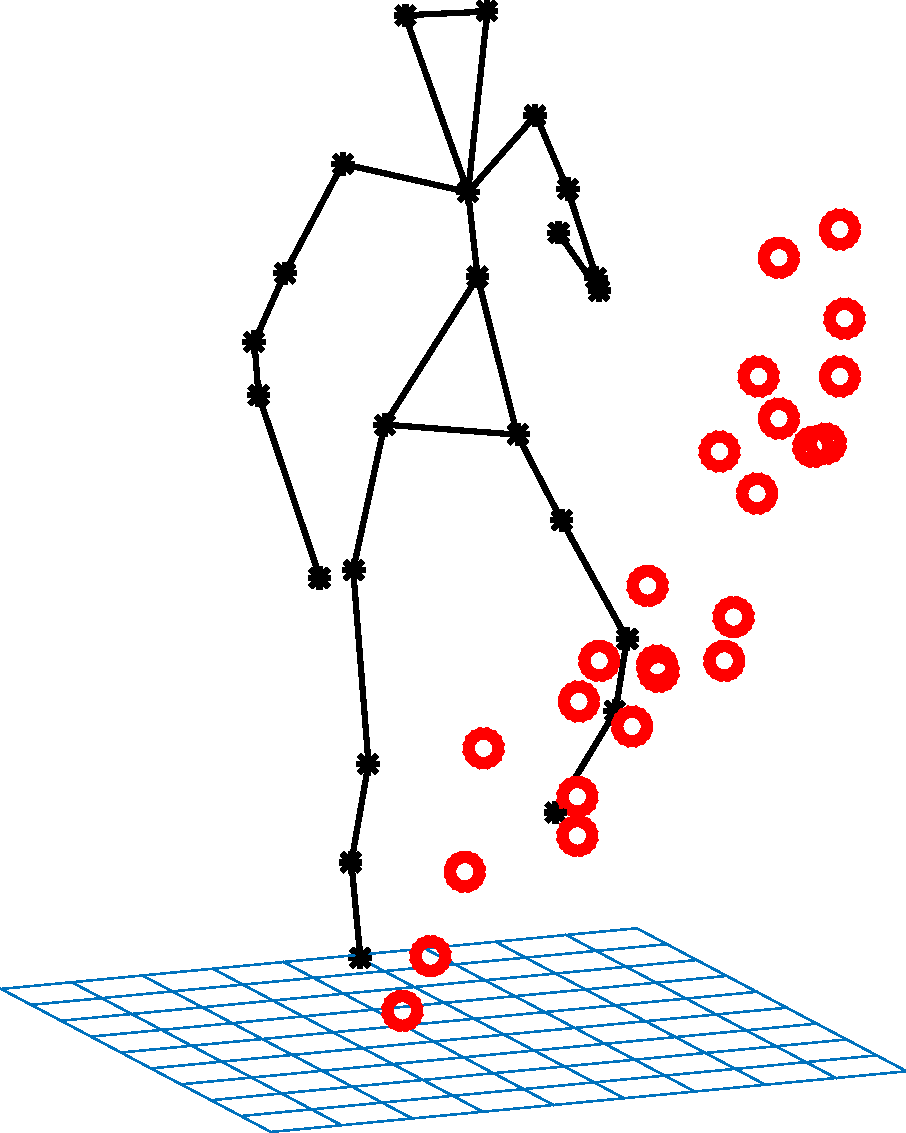
\includegraphics[width=0.155\textwidth]{chapter5/resource/compare_with_prior_free/priorfree/0091.pdf}
\label{fig:prior_free_Qualitative_result}
}\\
\subfloat[General trajectory prior method \cite{Valmadre_CVPR2012} produces large errors due to high system condition ($1/\sigma_{\text{min}}=2228$)]{
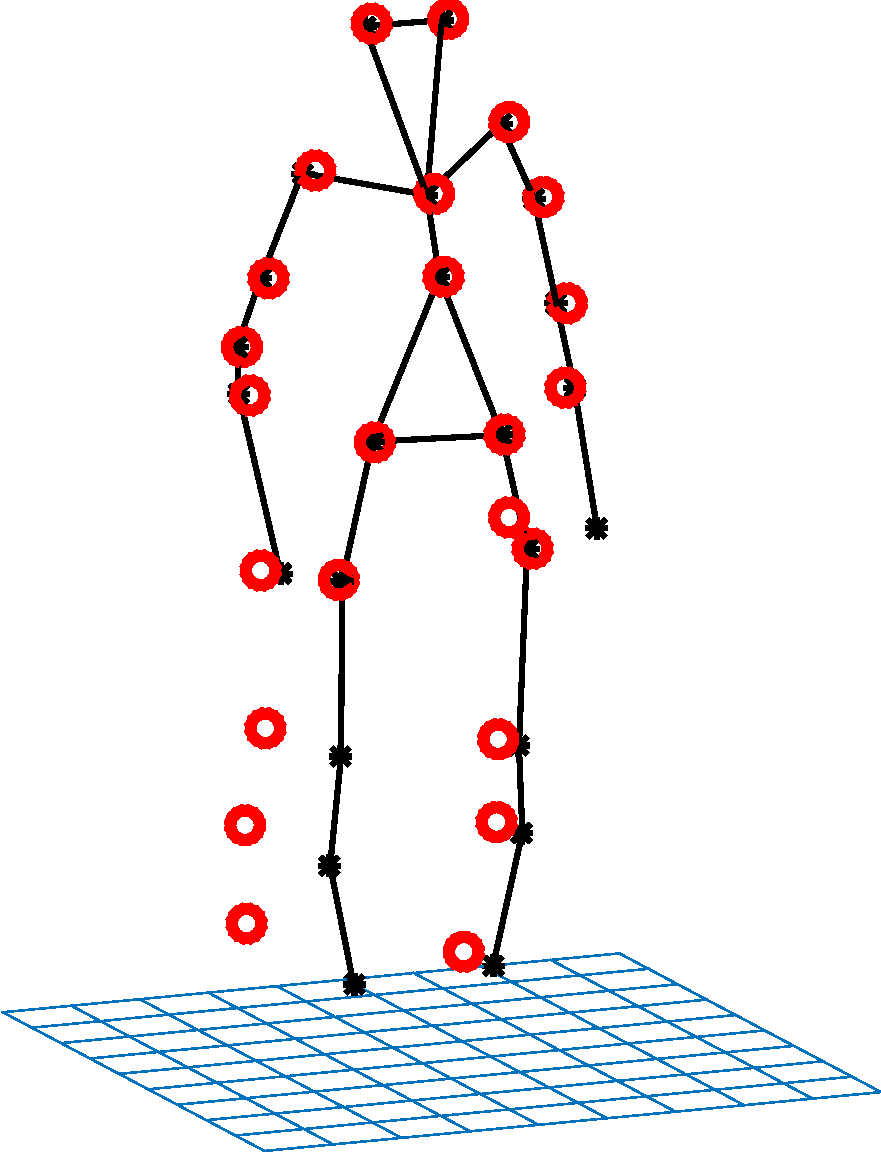
\includegraphics[width=0.155\textwidth]{chapter5/resource/compare_with_prior_free/filtermethod/0001.pdf}
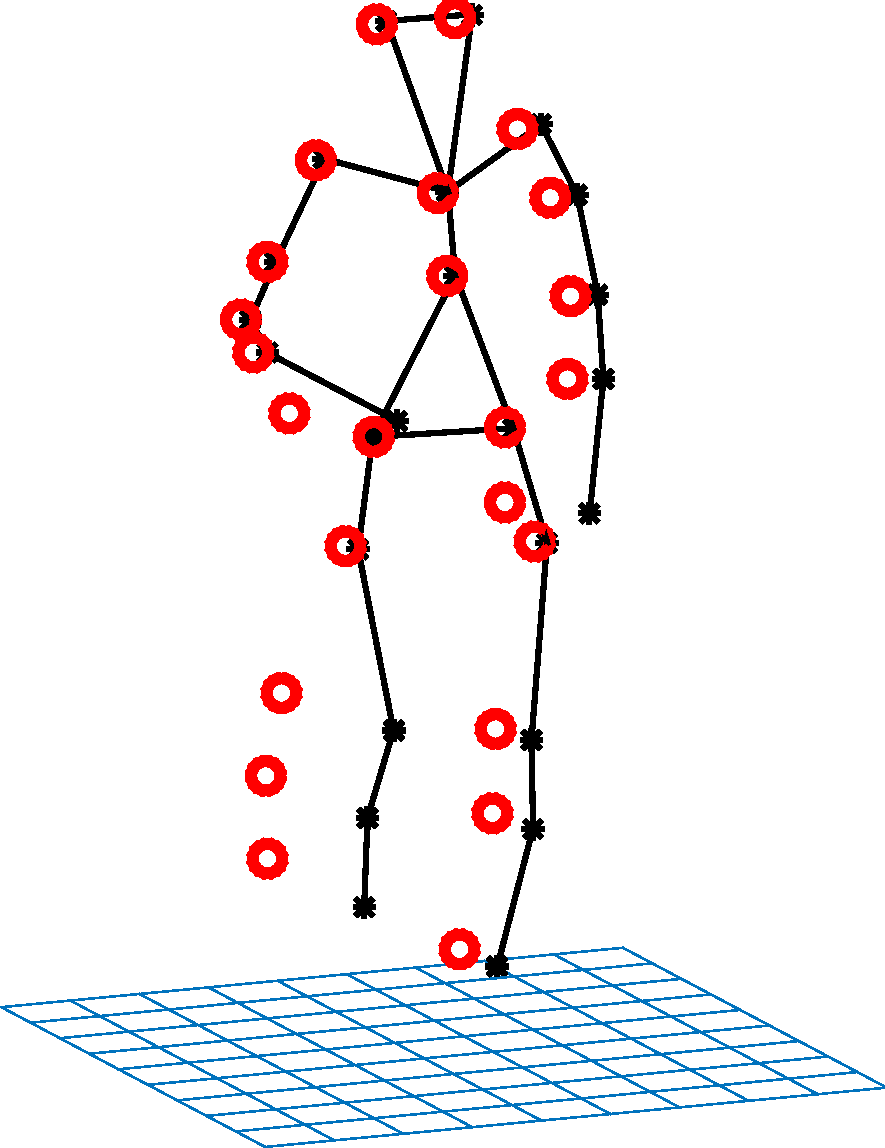
\includegraphics[width=0.155\textwidth]{chapter5/resource/compare_with_prior_free/filtermethod/0033.pdf}
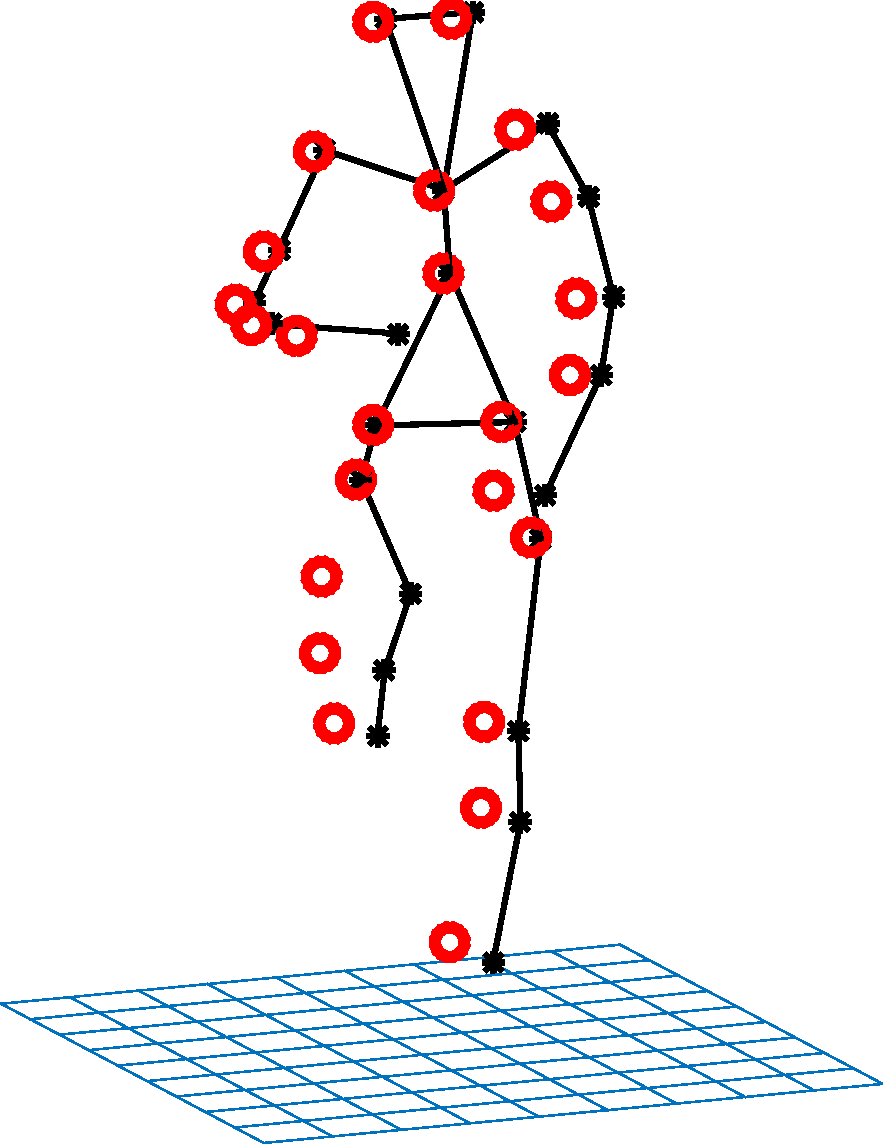
\includegraphics[width=0.155\textwidth]{chapter5/resource/compare_with_prior_free/filtermethod/0055.pdf}
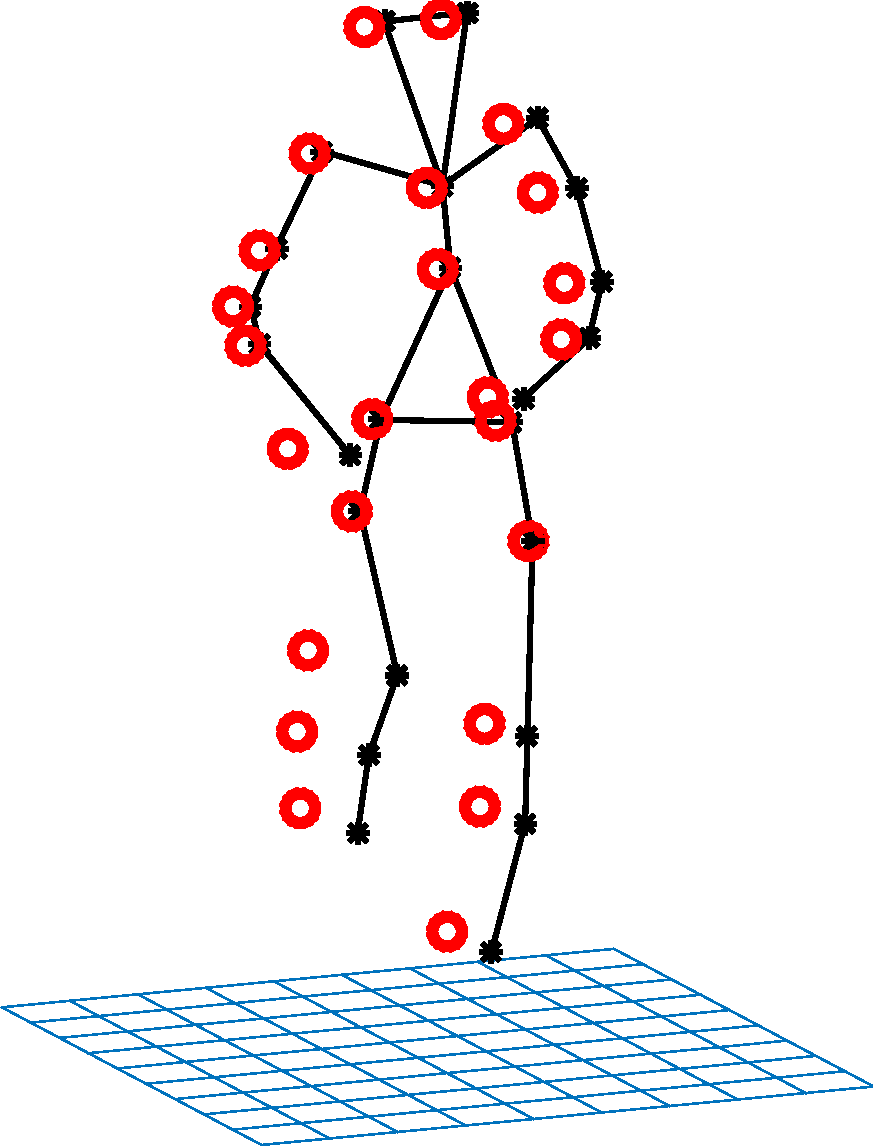
\includegraphics[width=0.155\textwidth]{chapter5/resource/compare_with_prior_free/filtermethod/0069.pdf}
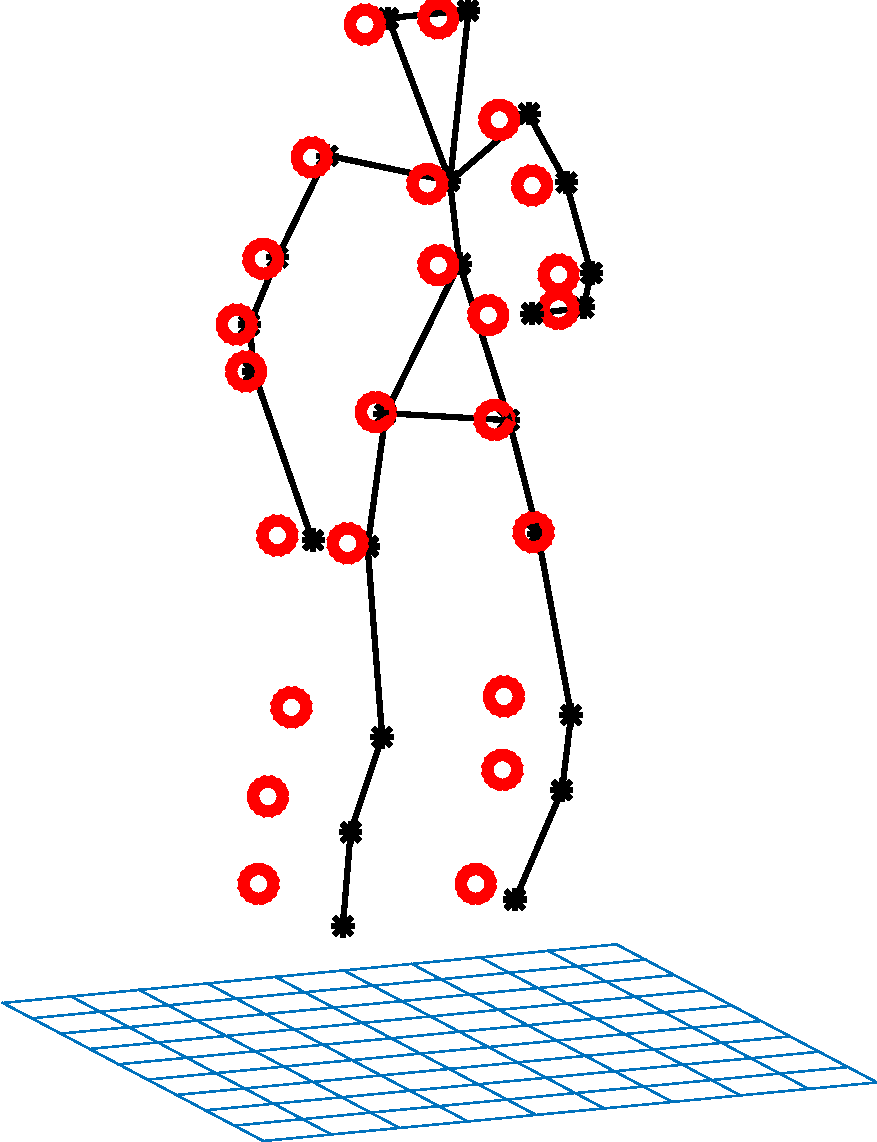
\includegraphics[width=0.155\textwidth]{chapter5/resource/compare_with_prior_free/filtermethod/0079.pdf}
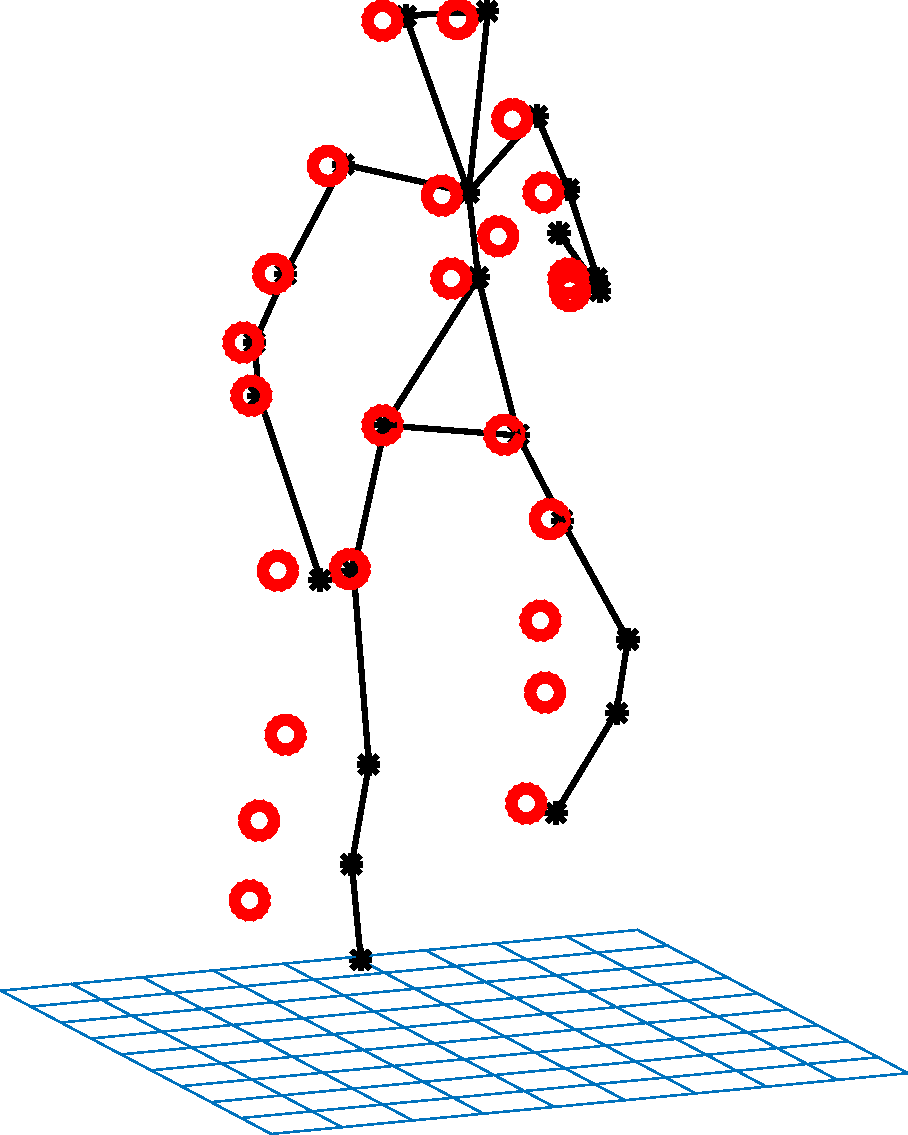
\includegraphics[width=0.155\textwidth]{chapter5/resource/compare_with_prior_free/filtermethod/0091.pdf}
\label{fig:trajectory_Qualitative_result}
}
\caption{Qualitative comparison of our method with \cite{dai2014simple} and \cite{Valmadre_CVPR2012} on the motion capture dataset `jog on place' in \cite{cg-2007-2}. The dataset has 214 frames, with 44 points per frame (only 24 are shown for visualization purposes). The black and red points are the ground truth and the estimated results, respectively. The average error per point for the three methods are (a) 0.0825, (b) 472.9033, and (c) 76.9700.}
\end{figure}

\textbf{Trajectory Triangulation Method.} We also compare with the trajectory triangulation method by  \citet{Valmadre_CVPR2012}, as is described in Section \ref{sec:importance_of_image_sequencing}. 
Since the required sequencing information is readily available within each video stream, our test uses the simulation of one handheld camera as shown in Figure \ref{fig:oneCam}. The camera centers are Gaussian with 20 mm standard deviation ($\sigma_c$) around a fixed point. %The larger the standard deviation, the better the reconstructability. 
Based on the theory in Section \ref{sec:system_condition}, the reconstructability increases with larger $\sigma_c$.
Considering that the framerate of the motion capture dataset is 120 Hz, the camera motion with  $\sigma_c = 20$mm is already very large compared to real handheld captures.

The method triangulates the trajectory of each dynamic point independently, and 
each trajectory has one system condition given the viewing ray directions. 
Since the motion of the person's head is relatively slower than that of his legs, the corresponding system condition is lower and the reconstructed points are more accurate, based on the theory in Section \ref{sec:system_condition}. 
The average system condition for all the points is 2228. 
Figure \ref{fig:trajectory_Qualitative_result} shows the large system condition in this camera setup leads to significant reconstruction errors.

\subsection{Real Datasets}
\begin{figure*}
\centering
\subfloat[Rothman dataset (250 frames)]{
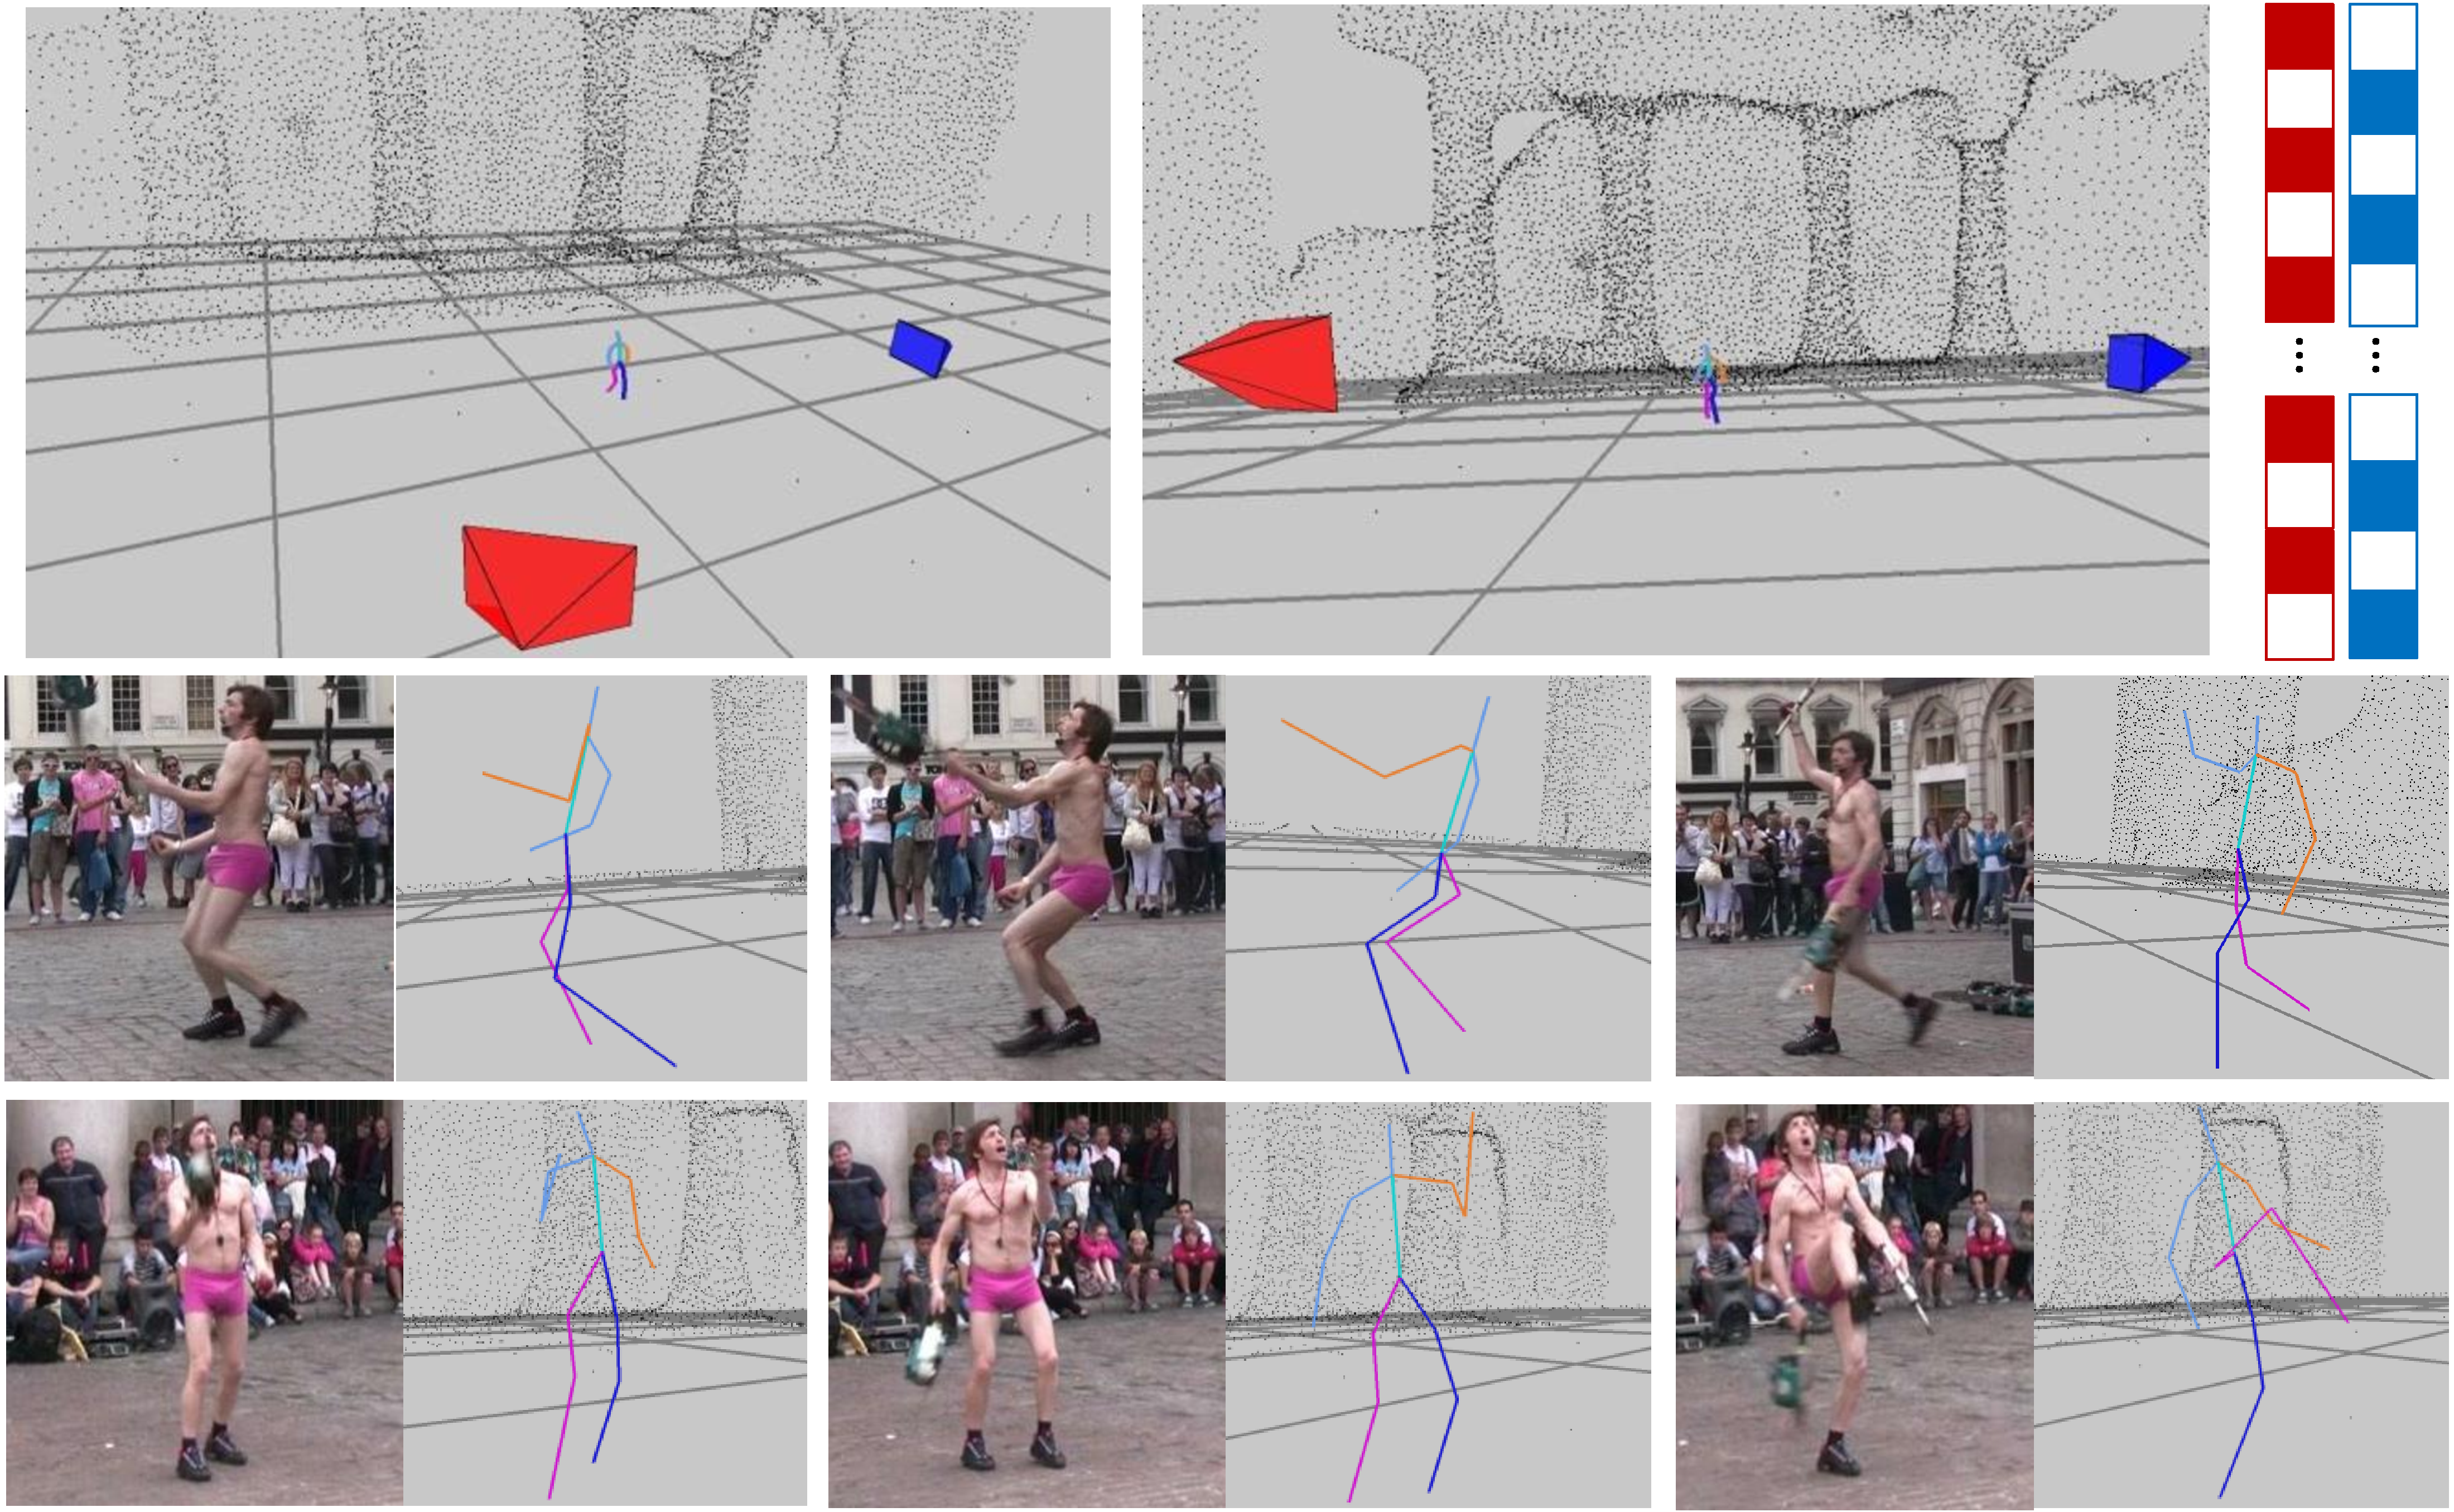
\includegraphics[width=0.94\textwidth]{chapter5/resource/2_pdfsam_image_cropped.pdf} 
}

\subfloat[Juggler dataset (180 frames)]{
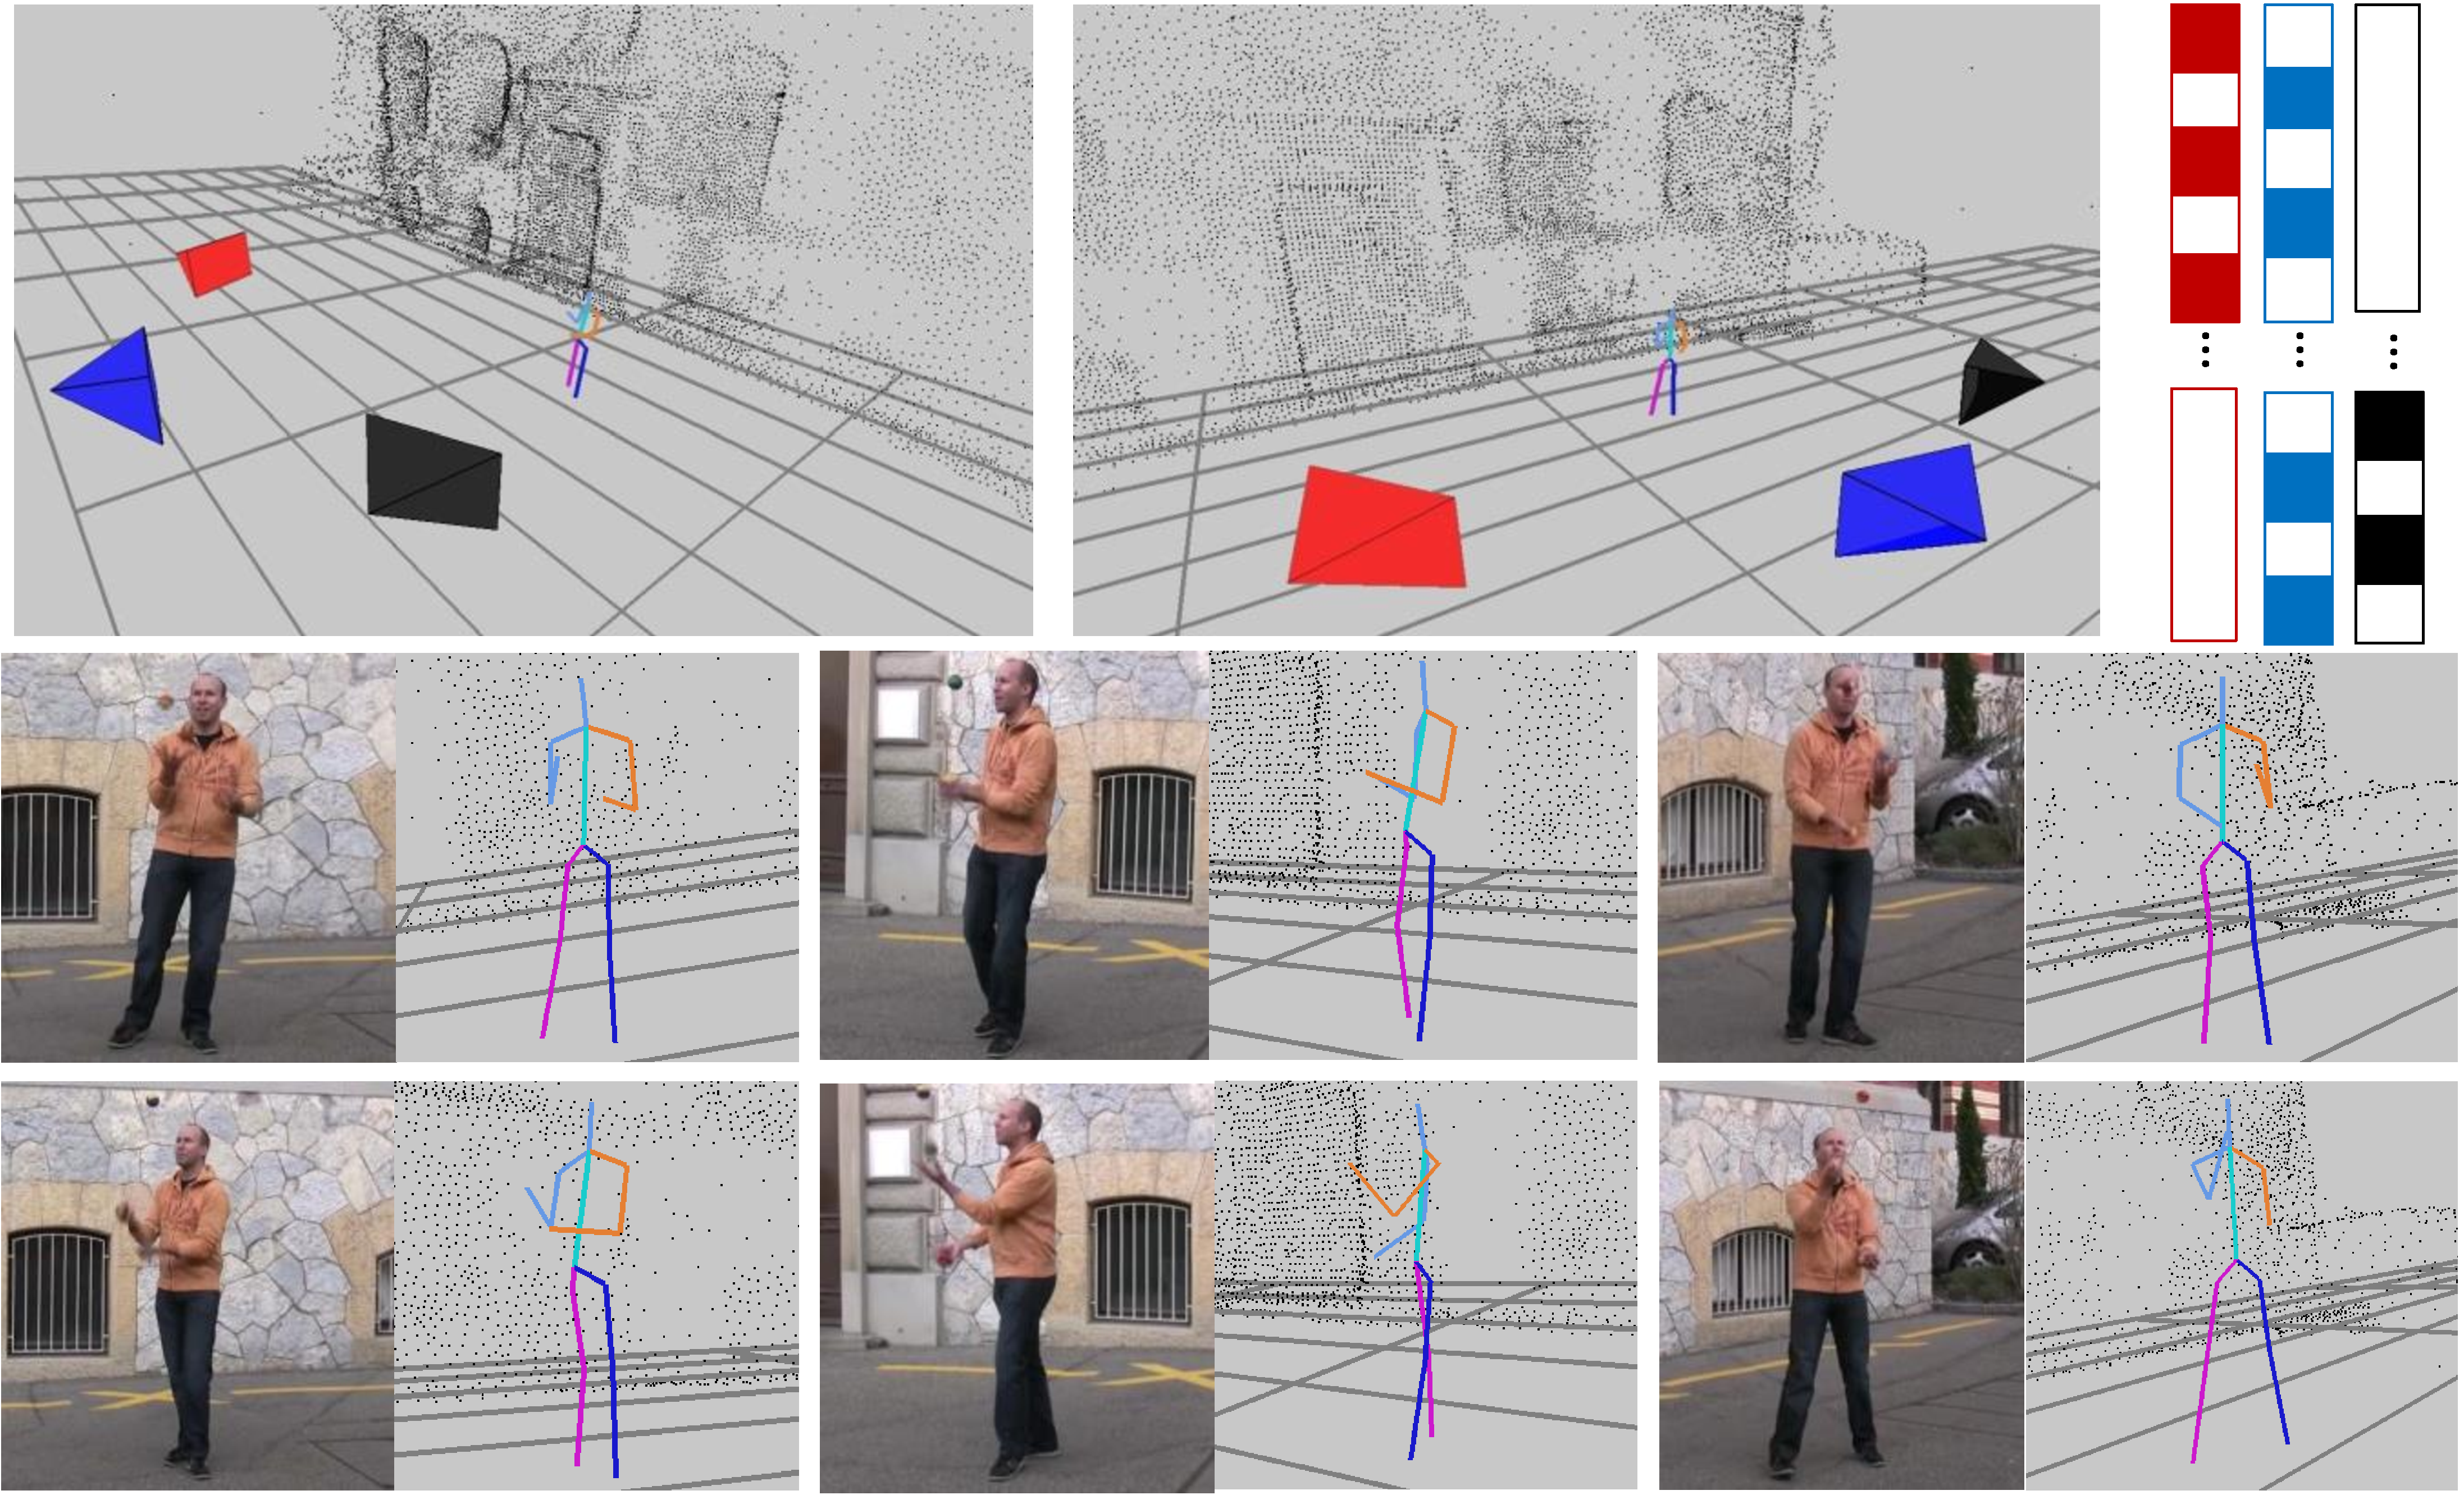
\includegraphics[width=0.94\textwidth]{chapter5/resource/1_pdfsam_image_cropped.pdf}
}
\caption{The datasets presented in \cite{ballan2010unstructured}. The frame rate of each camera is 12.5 Hz. For each dataset, the top left two show the camera configuration, the top right describes the temporal distribution of each image sequence (a colored grid means the camera of the same color captures one frame at a time instance), and the bottom shows sample reconstruction results. }
\label{fig:onlinedata}
\end{figure*}

\begin{figure*}
\centering
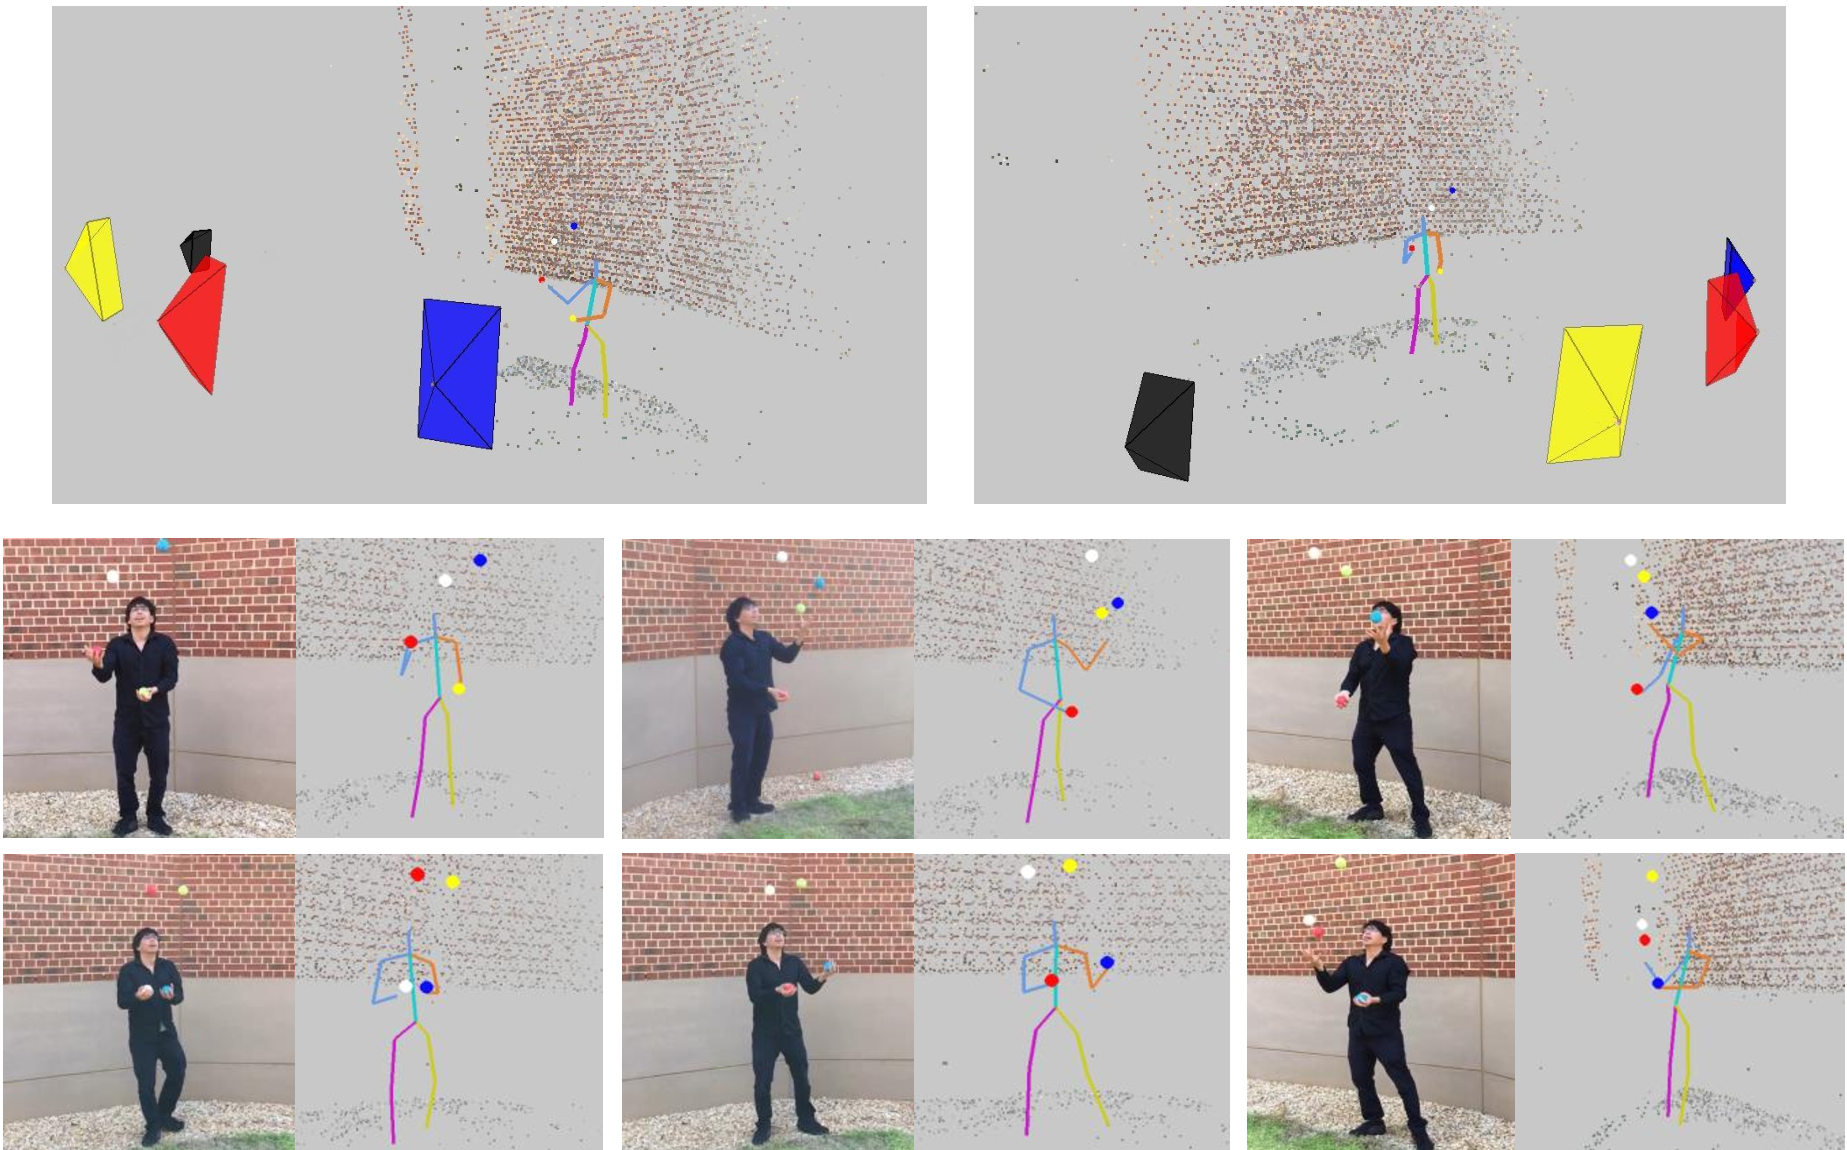
\includegraphics[width=0.92\textwidth]{chapter5/resource/3_pdfsam_image_cropped.pdf}
\caption{Results of a person juggling. Note we reconstruct the four juggler balls in addition to the person. The image sequence from iPhone6 and iPhone5 have frame rates of 10 Hz and 6.25 Hz respectively}
\label{fig:juggler2}
\end{figure*}
For experiments on real image capture, we use the Juggler and Rothman datasets from \cite{ballan2010unstructured}. Given that the original datasets were synchronized, we sample the video frames to avoid concurrent captures (see Figure \ref{fig:onlinedata}). 
We do not use the datasets in the work by \citet{Basha_ECCV2012,Park_ECCV2010} because they only provide images with large temporal discrepancy, and therefore the shape residual is large (\ie~Equation (\ref{eq:linear_comb_2}) does not hold). We also capture a new dataset of a person juggling using three iPhone6 and one iPhone5 without temporal synchronization. 

%The camera poses and internal calibration are provided for both of these datasets.
We perform manual feature labeling on the input sequences and provide the obtained set of 2D measurements as input for our estimation process.
For visualization purposes, Figures \ref{fig:onlinedata} and \ref{fig:juggler2} depict the estimated 3D geometry by connecting the estimated position of the detected joint elements through 3D line segments. 


\section{Conclusion and Contributions} \label{sec:conclusion_l1}
We have presented a method for dynamic object reconstruction from unsynchronized video streams. 
We demonstrated the effectiveness of our proposed method on both real and synthetic datasets.   This is a first step towards dynamic 3D modeling in the wild.

%Our proposed method was successfully evaluated on both real and synthetic data.

The main contributions of our approach encompass:
\begin{enumerate}%[topsep=-1ex,itemsep=-1ex,partopsep=1ex,parsep=1ex]
\item {\bf Problem Definition}. We are the first to address the problem of dynamic 3D reconstruction using unsynchronized cross-video streams.
\item {\bf Methodology Formulation}. We pose the problem in terms of a self-expressive dictionary learning framework leveraging a novel data-adaptive local 3D interpolation model.  
\item {\bf Implementation Mechanisms}. We define and solve a biconvex optimization problem and develop an efficient ADMM-based solver amenable for parallel implementation.
\end{enumerate}
To the best of our knowledge, we are the first to use the self-expression prior to solve the problem of dynamic object reconstruction. This prior has the potential to be applied in the traditional NRSFM problems.
%for which most of the existing methods make use of the assumption of representing shapes using a fixed number ($K$) of shape bases\cite{Bregler_CVPR2000,Xiao_ECCV2004,torresani2008nonrigid,dai2014simple}.  




